\documentclass[a4paper,11pt,oneside]{report}
\usepackage[utf8]{inputenc}
\usepackage{graphicx}
\usepackage{amsmath}
\usepackage{amsthm}
\usepackage{amsfonts}

\newtheoremstyle{named}{\topsep}{\topsep}{\itshape}{0pt}{\bfseries}{\vspace{\baselineskip}}{\newline}{\thmnote{#3}}
\theoremstyle{named}
\newtheorem{named}{Theorem}[section]

\usepackage[labelfont=bf]{caption}
\usepackage{hyperref}

\addtolength{\topmargin}{-20pt}
\addtolength{\textheight}{40pt}

\title{\textbf{Reconstruction of composite sparse-plus-smooth images using mixed penalties} \\[2ex] \large Bachelor Project - Spring 2022}
\author{David Rochinha Chaves\\{\small Supervisor: Adrian Jarret}\\[2cm]{AudioVisual Communications Laboratory - EPFL}}
\date{

\includegraphics[width=2.9in]{EPFLlogo}

\includegraphics[width=2.2in]{LABlogo}}

\begin{document}

\maketitle
\tableofcontents

\chapter{Introduction}
The objective of the project is to write a python framework that solves discrete linear inverse problems on 2D composite sparse-plus-smooth signals. These signals are the sum of two components, a sparse one and the other one smooth. The goal is to reconstruct these type of signals given a number of linear measurements, and then to also study how this model works and compare to preexisting ones, i.e. Lasso and Tikhonov. We apply this model in the domain of radio astronomy where the signals are images, with 2D Fourier measurements. The motivation of this project follows from \cite{formulation} where the continuous-domain analog regularized inverse problem is formulated. It presents and proves the representer theorem for the mixed penalty minimization problem approach used here.

In this work, we code in python with the package \href{https://github.com/matthieumeo/pycsou}{pycsou} \cite{matthieu_simeoni_2021_4715243}, a solver for reconstructing images. Then we use it with simulated signals to test the performance and see the impact of each parameter. Finally we test the framework on real world images.


\chapter{Model}
In this section we will present the model we consider, how it can be solved via a minimization problem and study the form of the solutions given by the representer theorem.

\section{Inverse problem}

The goal is to reconstruct some signal $\boldsymbol{x} \in \mathbb{R}^N$ from his linear measurements $\boldsymbol{y} \in \mathbb{C}^M$ such reconstruction is called an inverse problem. The relationship is as follow
\begin{equation}
    \boldsymbol{y} = \boldsymbol{H x} + \boldsymbol{Z}, \hspace{10pt} \boldsymbol{Z} \sim \mathbb{C} \mathcal{N}(0, \sigma^2 \boldsymbol{I}_M)
\end{equation}
where $\boldsymbol{y}$ is our measurements given from a linear measurement operator $\boldsymbol{H}$ with some additive white Gaussian noise, $\boldsymbol{Z}$. \\
The specificity in our case is that $\boldsymbol{x}$ is a sparse-plus-smooth signals and can be decompose as $\boldsymbol{x} = \boldsymbol{x}_1 + \boldsymbol{x}_2$ where $\boldsymbol{x}_1$ is sparse, i.e. $\boldsymbol{x}_1$  has a few non-zero values and $\boldsymbol{x}_2$ is smooth. It gives us 
\begin{equation} \label{eq:1}
    \boldsymbol{y} = \boldsymbol{H x}_1 + \boldsymbol{H x}_2 + \boldsymbol{Z}, \hspace{10pt} \boldsymbol{Z} \sim \mathbb{C} \mathcal{N}(0, \sigma^2 \boldsymbol{I}_M)
\end{equation}

More specifically, $\boldsymbol{x}$ is an image which give us a discrete problem and takes away the issues of working in the Continuous-Domain. Our measurement operator $\boldsymbol{H}$ is the discrete Fourier transform (DFT), precisely the 2D discrete Fourier transform since we work with 2D signals. The domain of $\boldsymbol{H}$ is as follow \( \boldsymbol{H} : \mathbb{R}^N \xrightarrow{} \mathbb{C}^M\) where $N$ is the number of pixels, $M$ the number of measurements and $M < N$, we select M selected frequency to sample.

 The approach we have chosen to the solve this inverse problem, is by solving a minimization problem.

\section{Minimization problem}
By mean of a minimization problem, we aims at minimizing the discrepancy between the measurements $\boldsymbol{H x}$ of the reconstructed signal $\boldsymbol{x}$ and the acquired measurements $\boldsymbol{y}$. This data fidelity is measured with a convex loss function, in our case we use a least-squares functional, because it is the likelihood of the data $\boldsymbol{y}$ with additive white Gaussian noise. Then we need to add a regularization term for multiple reasons:

\begin{enumerate}
    \item to favor certain forms of reconstructed signal (e.g., sparse or smooth)
    \item to favor well-behave solutions, because different signals have identical measurements, indeed we have a underdetermined system that has a infinite number of solutions
    \item to improve the conditioning of the problem and thus increase its numerical stability
    \item to have robustness to noise
\end{enumerate}

To solve \eqref{eq:1} we use the following minimization problem

\begin{equation} \label{eq:min}
    \min_{\boldsymbol{x}_1,\boldsymbol{x}_2 \in \mathbb{R}^N} \frac{1}{2} ||\boldsymbol{H x}_1 + \boldsymbol{H x}_2 - \boldsymbol{y}||_2^2 + \lambda_1 ||\boldsymbol{L}_1 \boldsymbol{x}_1||_1 + \lambda_2 ||\boldsymbol{L}_2 \boldsymbol{x}_2||_2^2
\end{equation}
where $\boldsymbol{x}_1$, $\boldsymbol{x}_2$ are the two components of the signal $\boldsymbol{x} = \boldsymbol{x}_1 + \boldsymbol{x}_2$, $\lambda_1, \lambda_2 > 0$ are tuning parameters, $\boldsymbol{L}_1$ and $\boldsymbol{L}_2$ are two operator that describe the form of the solutions $\boldsymbol{x}_1$ and $\boldsymbol{x}_2$.

In our case we want the sparsity on $\boldsymbol{x}_1$ and not some linear transformation of $\boldsymbol{x}_1$, so $\boldsymbol{L}_1$ is the identity operator. We want $\boldsymbol{x}_2$ to be smooth, so $\boldsymbol{L}_2$ need to be a smoothing 
operator generally obtain with a differential operator, in our case we took the discrete Laplacian $\boldsymbol{\nabla}^2$. Our optimization problem becomes

\begin{equation} \label{eq:2}
    \min_{\boldsymbol{x}_1,\boldsymbol{x}_2 \in \mathbb{R}^N} \frac{1}{2} ||\boldsymbol{H x}_1 + \boldsymbol{H x}_2 - \boldsymbol{y}||_2^2 + \lambda_1 ||\boldsymbol{x}_1||_1 + \lambda_2 || \boldsymbol{\nabla}^2 \boldsymbol{x}_2||_2^2
\end{equation}

\section{Representer Theorem}
As discussed before the reason we choose to solve the inverse problem by solving a 
minimization problem, is because the form of the solutions are well known and stated by 
the Representer Theorem. We will now look at this Representer Theorem for Tikhonov 
Regularization and TV Regularization \cite{Slides}.

\begin{named}[Representer Theorem I: (TV Regularization)] \label{rep1}

Given that 
\begin{enumerate}
    \item $\boldsymbol{G} \in \mathbb{R}^{M \times N}$ is surjective, $\boldsymbol{D}$ is positive semi-definite and $\mathcal{N}(\boldsymbol{G}) \cap \mathcal{N}(\boldsymbol{D}) = \boldsymbol{0}$.
    \item $F(\boldsymbol{y}, \cdot) : \mathbb{R}^M \xrightarrow{} \mathbb{R}_+$ is proper convex, coercive and lower semi-continuous for every $\boldsymbol{y} \in \mathbb{R}^M$.
\end{enumerate}
Then the optimisation problem:
\begin{equation*}
    \min_{\boldsymbol{\alpha} \in \mathbb{R}^N} F(\boldsymbol{y}, \boldsymbol{G} \boldsymbol{\alpha}) + \lambda ||\boldsymbol{D \alpha} ||_1
\end{equation*}
admits solutions of the form:
\begin{equation*}
    \boldsymbol{\alpha} = \boldsymbol{D}^\dagger \boldsymbol{\beta}_K + \boldsymbol{\gamma},
\end{equation*}
for some K-sparse vector $\boldsymbol{\beta}_K \in \mathbb{R}^N$, $K\leq M$ and $\boldsymbol{\gamma} \in \mathcal{N}(\boldsymbol{D})$. Where $\boldsymbol{D}^\dagger$ is the pseudoinverse of $\boldsymbol{D}$

\end{named}


\begin{named}[Representer Theorem II: (generalised Tikhonov Regularization)] \label{rep2}

Given that 
\begin{enumerate}
    \item $\boldsymbol{G} \in \mathbb{R}^{M \times N}$ is surjective, $\boldsymbol{D}$ is positive semi-definite and $\mathcal{N}(\boldsymbol{G}) \cap \mathcal{N}(\boldsymbol{D}) = \boldsymbol{0}$.
    \item $F(\boldsymbol{y}, \cdot) : \mathbb{R}^M \xrightarrow{} \mathbb{R}_+$ is proper strictly convex, coercive and lower semi-continuous for every $\boldsymbol{y} \in \mathbb{R}^M$.
\end{enumerate}
Then the optimisation problem:
\begin{equation*}
    \min_{\boldsymbol{\alpha} \in \mathbb{R}^N} F(\boldsymbol{y}, \boldsymbol{G} \boldsymbol{\alpha}) + \lambda ||\boldsymbol{D \alpha} ||_2^2
\end{equation*}
admits a unique solution which can be written as
\begin{equation*}
    \boldsymbol{\alpha} = (\boldsymbol{D}^T\boldsymbol{D})^\dagger \boldsymbol{G}^T \boldsymbol{\beta} + \boldsymbol{\gamma},
\end{equation*}
for some $\boldsymbol{\beta} \in \mathbb{R}^M$ and $\boldsymbol{\gamma} \in \mathcal{N}(\boldsymbol{D})$.

\end{named}

The main motivation of using the composite model \eqref{eq:min} is that the two representer theorems presented can be combined into a composite one \cite{formulation} with a mixed penalty in the minimisation problem, so that can have the form of the solution describe by each representer theorem for each solution.

More specifically, it tells us that there exist $\boldsymbol{x} = \boldsymbol{x}_1 + \boldsymbol{x}_2$ such that $\boldsymbol{x}$ is solution of \eqref{eq:min}, $\boldsymbol{x}_1$ is  given by Representer Theorem I and $\boldsymbol{x}_2$ is given by Representer Theorem II. 

For \eqref{eq:2} we have $\boldsymbol{x}_1 = \boldsymbol{D}^\dagger \boldsymbol{\beta}_K + \boldsymbol{\gamma}$. With $\boldsymbol{D} = \boldsymbol{I}_N$, we obtain
\begin{equation} \label{x1}
    \boldsymbol{x}_1 = \boldsymbol{\beta}_K,
\end{equation}
for some K-sparse vector $\boldsymbol{\beta}_K \in \mathbb{R}^N$, $K\leq M$. So our vector $\boldsymbol{x}_1$ is a sparse vector with at most M non-zero component for M measurements. We see right away that if we wanted to solve \eqref{eq:1} with only a L1 penalty term, we could only recover M pixel of the image $\boldsymbol{x}$. Since $\boldsymbol{x}$ is dense, it means that using this we cannot obtain a good reconstruction. Along this we also emphasize that the sparse component does not depend on the measurement operator $\boldsymbol{H}$, but only on the number of measurements taken, which corresponds to the number of lines of $\boldsymbol{H}$. 

For the smooth component of \ref{eq:2}, the Representer Theorem II gives us $\boldsymbol{x}_2 = (\boldsymbol{D}^T\boldsymbol{D})^\dagger \boldsymbol{G}^T \boldsymbol{\beta} + \boldsymbol{\gamma}$ with $\boldsymbol{D} = \boldsymbol{\nabla}^2$. The discrete Laplacian $\boldsymbol{\nabla}^2$ is a self-adjoint ($D^T = D^{-1}$) and invertible operator, so we have
\begin{equation} \label{x2}
    \boldsymbol{x}_2 = \boldsymbol{D}^{-2} \boldsymbol{H}^T \boldsymbol{\beta} + \boldsymbol{\gamma}
\end{equation}
for some $\boldsymbol{\beta} \in \mathbb{R}^M$, $\boldsymbol{D} = \boldsymbol{\nabla}^2$ and $\boldsymbol{\gamma} \in \mathcal{N}(\boldsymbol{D})$. This solution is not as straightforward to understand as before. First we have $\boldsymbol{\gamma}$ in the null space of the Laplacian, which is some paraboloid that is smooth as wanted. $\boldsymbol{H}^T \boldsymbol{\beta}$ is the inverse Fourier transform of some measurement's vector, which give us an image. Then we have $\boldsymbol{D} ^{-2} = \boldsymbol{\nabla}^{-4}$ which we can see as applying a fourth order integration, which is a smoothing operator, on $\boldsymbol{H}^T \boldsymbol{\beta}$. So $\boldsymbol{x}_2$ is just the integration of some image, plus some base smooth vector, which give us a smooth $\boldsymbol{x}_2$. To have a better idea of what $\boldsymbol{\nabla}^{-4}$ actually mean, we can look at it in the other way, when we have the penalty term $||\boldsymbol{\nabla}^2 \boldsymbol{x}_2||_2^2$ in the minimisation problem, we are telling that the second order derivative of $\boldsymbol{x}_2$ is a vector with minimum L2 norm. So the vector $\boldsymbol{x}_2$ needs to be "smooth enough" for his derivative to be "small", the nearest possible to zero. For example if we take a non-smooth image, it means that the pixel values change very quickly in space then his derivative will be big. With the use of the Laplacian, we are further telling that we want a image composed of paraboloids, since those have a Laplacian of zero.

\section{Measurements}

\subsection{Measurement methods} \label{methods}
In this section we present how the measurements $\boldsymbol{y}$ simulated. As say before the measurements are done with a 2D DFT, that we call Fourier measurements. What we do is that we take the measurements $\boldsymbol{y}$ as the subsampling of the Fourier measurements of the input image with N pixels, we sample M pixels out of N, $M < N$. 

To chose those M measurements, we present 3 following methods shown in the Figure \ref{fig:samp}:

\begin{itemize}
    \item Sampling the highest Fourier coefficients (b)
    \item Uniform sampling, each pixel has the same chance to be sample (c)
    \item Our custom "Gaussian + Uniform" sampling (d)
\end{itemize}

On Figure \ref{fig:samp} (a) we show the 2D DFT of our simulated signal, i.e. the Fourier measurements that we subsample. The uniform method (c) has a fundamental problem, our image is not uniform in the frequency domain, we have a some important low frequency coefficients. We need a good number of these important measurements to be able to reconstruct the smooth component correctly. We also have another problem, in reality the measurements we can take in radio astronomy are not uniform either. To model better this scenario, we opted for a model which assign more chance to sample low frequency measurement, called "Gaussian + Uniform" shown in the figure \ref{fig:samp} (d). We have sample the image with a 2D Multivariate normal distribution so that we have a more realistic way of sampling, but by doing this we will never sample the edges of the image. The sparse component has a Fourier transform that is spread though all frequency so the best sampling method for it, is the Uniform (c). The Uniform in (d) comes from this previously stated fact, that even though our image is sparse in frequency, we need some sampling of all frequencies to reconstruct our sparse component. If we compare our measurement's method to what we could call the best measurements, the highest Fourier coefficients (b) we have something very similar. (b) measures all important low frequency measurements due to the smooth component and then it takes a uniform sampling of the rest for the sparse component.

\begin{figure}[t]
    \centering
    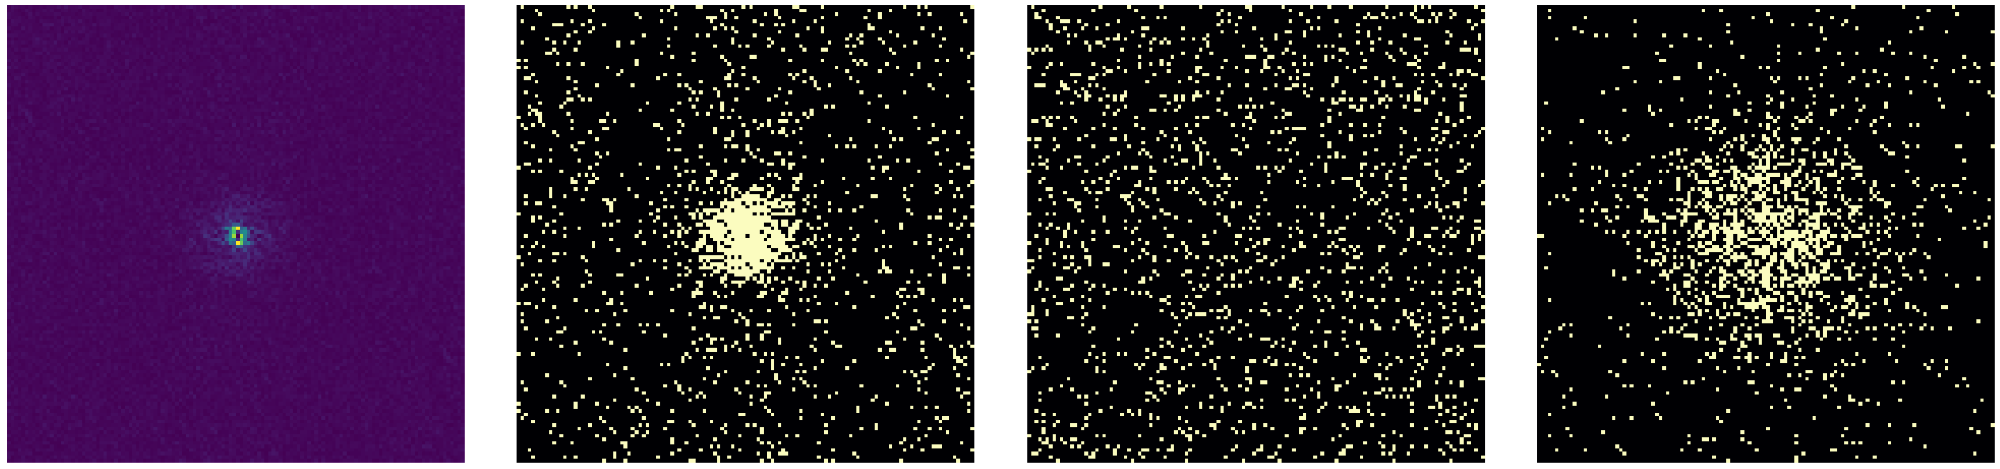
\includegraphics[width=1\textwidth]{Sampling_methods_comparison.png}
    \setlength{\tabcolsep}{39pt}
     \begin{tabular}{c c c c}
         (a) & (b) & (c) & (d)
    \end{tabular}
    \caption{\textbf{Measurement methods with 10\% of the image}\\(a) Show the magnitude of the Fourier transform of our simulated signal. \\ (b) Highest Fourier coefficients of (a). (c) Uniform sampling. (d) Our "Gaussian + Uniform" sampling}
    \label{fig:samp}
\end{figure}

\subsection{0-frequency}

Another important point about the measurements is the frequency 0, this is important because it tells us the mean value of the signal. In radio astronomy, we do not take this 0-frequency measurement because he is too noisy to work with. So we will do the same thing here and exclude the 0-frequency from our measurements. By doing this we will have the two components of our signal $\boldsymbol{x}$ to have 0-mean which is not what we want since both are positive (i.e. the image measure the intensity of light so it can only be 0 or a positive value). For the sparse one there is not much problem since the only thing that the optimizer does is adding some small negative coefficient. Those are easy to solve we can just set those negative values to zero. For the smooth component we have a bigger problem since a 0-mean image means that our signal will be centred around 0, with negative and positive values. One way to solve this, is to offset the image by some value, but what value to choose ? A natural one is to offset by the minimum value so that we have a positive signal, but this is not a good idea since this minimum value is often really low on the edges of the image due to edge effect with the Laplacian, which then gives a image that is a lot higher than the original one. A better one is to offset it by the mean value of the true smooth component, which makes the reconstruction to have the same mean as the original. But the main problem of this is that it requires to have access to original image, which is not the case is practise. The solution we have opted for is to add a positivity constraint on the smooth component $\boldsymbol{x}_2$, which works well in practise as shown in chapter \ref{Results}. Another point is that adding this constraint cost us almost nothing in the implementation and in the performance as we will see in chapter \ref{imp}. Why not add a positivity constraint on the whole signal, two reasons. First the implementation of this slow down the performance considerably and second is gives worse results for the sparse component compare to only using it on the smooth one, it makes the sparse component lose a lot of energy. And since for the sparse component we can easily remove the negative values, these is no point is adding a useless positivity constraint.

\chapter{Implementation}\label{imp}
In this section we will talk about how we have implemented the solver for the minimization problem \eqref{eq:2} in Python. All the code is available on \href{https://github.com/Dado0x/Sparse-smooth-signal}{GitHub}.
\section{Getting started}
To implement the solver we have used the library \href{https://github.com/matthieumeo/pycsou}{pycsou} \cite{matthieu_simeoni_2021_4715243} which is a Python 3 package for solving linear inverse problems with proximal algorithms. The package is really help full because it implements in a highly modular way the main building blocks of convex optimisation problems, cost functionals, penalty terms, linear operators and the state-of-the-art proximal algorithms.

\subsection{Image to vector}
First of all we working with image in a linear problem, we have to ravel our images into a vector so that we can work with matrix and matrix multiplication. It is simply done by concatenate each line of the image into a vector. 

\subsection{Accelerated Proximal Gradient Descent}
To solver \eqref{eq:2} we use the Accelerated Proximal Gradient Descent (APGD) algorithm. We can use this algorith to solve problems of the form
\begin{equation*}
    \min_{\boldsymbol{x} \in \mathbb{R}^N} F(\boldsymbol{x}) + G(\boldsymbol{x})
\end{equation*}
where $F$ is convex and differentiable and $G$ is convex with a simple proximal operator. In our case $F$ contains the data fidelity term $||\boldsymbol{H x} - \boldsymbol{y}||_2^2$ and the L2 norm penalty term $|| \boldsymbol{\nabla}^2 \boldsymbol{x}_2||_2^2$, since the squared L2 norm is convex and differentiable. The term $G$ is the L1 norm penalty functional $||\boldsymbol{x}_1||_1$, which is convex and crucially has a simple proximal operator. If we where to have $G(\boldsymbol{x}) = ||\boldsymbol{D x}_1||_1$ with some operator $\boldsymbol{D}$ different from the identity $\boldsymbol{I}$, then we would not be able to use APGD. 

\subsection{Operator stacking}
We want to solve for $\boldsymbol{x}_1$, $\boldsymbol{x}_2$ and obtain two separate vectors, and not the sum $\boldsymbol{x}$. To do so with Pycsou, we need to stack the operators and penalty functionals we use. There is two ways to stack the vectors, horizontally and vertically. Vertical stacking is defined as $\boldsymbol{V}: \boldsymbol{x} \xrightarrow{} ( \boldsymbol{L}_1 \boldsymbol{x}, \dots, \boldsymbol{L}_k \boldsymbol{x} ) $ where we stack the collection $\{\boldsymbol{L}_1,\dots, \boldsymbol{L}_k\}$ of linear operators vertically. Horizontal stacking is defined as  $\boldsymbol{H}: (\boldsymbol{x}_1,\dots,\boldsymbol{x}_k) \xrightarrow{} \sum_{i = 1}^{k} \boldsymbol{L}_i \boldsymbol{x}_i$ where we stack the collection $\{\boldsymbol{L}_1,\dots, \boldsymbol{L}_k\}$ of linear operators horizontally. Clearly what we want is a horizontal stacking with the two vectors $\boldsymbol{x}_1$ and $\boldsymbol{x}_2$ as input.

\subsection{Solver implementation}
Now we have everything to code our solver. First we need to build $F(\boldsymbol{x}_1, \boldsymbol{x}_2)$ and $G(\boldsymbol{x}_1, \boldsymbol{x}_2)$ with the horizontal stacking then pass them as input into the APGD solver. Our APGD solve will solve
\begin{equation*}
    \min_{\boldsymbol{x}_1, \boldsymbol{x}_2 \in \mathbb{R}^N} F(\boldsymbol{x}_1, \boldsymbol{x}_2) + G(\boldsymbol{x}_1, \boldsymbol{x}_2)
\end{equation*}
with $F(\boldsymbol{x}_1, \boldsymbol{x}_2) = \frac{1}{2} ||\boldsymbol{H x}_1 + \boldsymbol{H x}_2 - \boldsymbol{y}||_2^2 + \lambda_2 || \boldsymbol{\nabla}^2 \boldsymbol{x}_2||_2^2$ and $G(\boldsymbol{x}_1, \boldsymbol{x}_2) = \lambda_1 ||\boldsymbol{x}_1||_1$.
Looking at the code for $\frac{1}{2} ||\boldsymbol{H x}_1 + \boldsymbol{H x}_2 - \boldsymbol{y}||_2^2$, we just have
\begin{verbatim}
stack_H = LinOpHStack(H, H)
l2_loss = (1 / 2) * SquaredL2Loss(H.shape[0], self.y)
F = l2_loss * stack
\end{verbatim}
where in the first line we stack the operator $\boldsymbol{H}$ horizontally, in the second line we create a squared L2 Loss operator that compute the following $\frac{1}{2} ||\boldsymbol{x} - \boldsymbol{y}||_2^2$ for input x and the third line is just a composition of the two maps to have the first one apply $\boldsymbol{x} = \boldsymbol{H x}_1 + \boldsymbol{H x}_2$ and then apply $F = \frac{1}{2} ||\boldsymbol{x} - \boldsymbol{y}||_2^2$. Now we just need to add $\lambda_2 || \boldsymbol{\nabla}^2 \boldsymbol{x}_2||_2^2$ to $F$. 
\begin{verbatim}
l2_operator = Laplacian(dim)
L2 = lambda2 * SquaredL2Norm(l2_operator.shape[0]) * l2_operator
F = F + DiffFuncHStack(NullDifferentiableFunctional(H.shape[1]), L2)
\end{verbatim}
where \verb+l2_operator+ is the discrete Laplacian for images for dimension \verb+dim+, it can be any other suitable linear operator. In the second line we do same as before, creating a squared L2 norm and doing the composition. Finally, we need to stack this with a null differentiable functional so that we have $\boldsymbol{x}_1$ evaluate to zero and also have the correct input dimension. 

Similarly for G, we have
\begin{verbatim}
G = ProxFuncHStack(self.lambda1 * L1Norm(H.shape[1]), 
                   NullProximableFunctional(H.shape[1]))
\end{verbatim}
where we stack the L1 functional with a null proximable functional. The only difference from $F$ is that we work with proximable functionals and not differentiable ones. 

Previously we said that we needed to  add a positivity constraint on $\boldsymbol{x}_2$, because we do not take the frequency 0 and claimed that this could be easily implemented. It is indeed the case since the positivity constraint is just a proximal operator. The proximable functional used for $\boldsymbol{x}_2$ in $G$, is the null one, so we can replace it with the NonNegativeOrthant fonction of Pycsou which enforce positive real solutions by evaluating negative inputs to infinity. G becomes
\begin{verbatim}
G = ProxFuncHStack( self.lambda1 * L1Norm(H.shape[1]), 
                    NonNegativeOrthant(H.shape[1]))
\end{verbatim}
To finish the APGD solver is
\begin{verbatim}
apgd = APGD(2 * H.shape[1], F=F, G=G, acceleration='CD')
\end{verbatim}
where \verb+2 * H.shape[1]+ is the size of $\boldsymbol{x}$ the variable for which we solve, $\boldsymbol{x}$ is implemented as the concatenation of $\boldsymbol{x}_1$ and $\boldsymbol{x}_2$. To retrieve the solutions we just do
\begin{verbatim}
estimate, converged, diagnostics = apgd.iterate()
x = estimate['iterand']
x1 = x[:H.shape[1]]
x2 = x[H.shape[1]:] 
\end{verbatim}

\section{Measurement operator}
We will now look at how we implement the linear operator $\boldsymbol{H}$ that does the 2D DFT, to be the most efficient possible in terms of memory and CPU utilisation. The first and naive approach is to use a matrix and do a matrix multiplication with the image vector. This approach was the first one we coded in \verb+SparseSmoothSignal.create_measurement_operator()+. To create this matrix we simply Fourier transform each canonical base vector of the image space of a given dimension. By concatenating the resulting image vectors in a matrix we get the wanted matrix where the matrix multiplication with a image vector gives us the 2D DFT of this image. 

This approach has two major problems, one is that it uses a lot of memory, since for an image for size $n \times m$, the full rank operator size is $nm \times nm$. For example with an image of $256 \times 256$ pixels, where each pixel is a 64-bit float values, we need 32GBs of memory just to store the operator. The second problem is that matrix multiplication is really slow and we have a better algorithm. 

The second approach and best solution is to use the fast Fourier transform since it is faster that matrix multiplication and is memory free. So we have implemented $H$ with the \verb+numpy.fft.fft2()+ function of numpy and  we call it matrix free operator. The operator is the class \verb+Solver.MyMatrixFree+  \verb+Operator+. We can do this since Pycsou supports these matrix-free operators. The implementation only consists on extending the class \verb+LinearOperator+ of Pycsou and then rewrite the two methods \verb+__call__()+ and \verb+adjoint()+. All the class' methods can be implemented in terms of these two.  The \verb+__call__()+ method is the forward pass, we just compute the DFT of the input $\boldsymbol{x}$ with \verb+np.fft.fft2()+ and then keep $M$ measurements. For \verb+adjoint()+ we have as input $\boldsymbol{y}$, the $M$ measurements and we need to output the image $\boldsymbol{x}$. To do so we first build a complete image from $\boldsymbol{y}$ where we have zeros on all pixel that are not measured and then we pass it though the inverse Fourier transform with \verb+np.fft.ifft2+. Like this we have implemented the operator H efficiently.

\section{Simulated signal}
Now that we have our solver we need to be able to test and analyse how it performs. To do it we need to build a simulated random test signal shown in \ref{fig:SpareSmoothSignal}. The implementation of our signal is the class \verb+SparseSmoothSignal+. Our signal is the sum of the sparse and smooth component. The sparse image is just an image where some pixel have a high value, compare to the smooth signal, from a uniform distribution and the rest of pixels are 0. To create this we simply use \verb+sparse.rand+ from Scipy as follow
\begin{verbatim}
sparse = scipy.sparse.rand(dim[0], dim[1], density=0.005)
sparse = (MAX_SPARSE_AMPLITUDE - MIN_SPARSE_AMPLITUDE) * sparse
sparse.data += MIN_SPARSE_AMPLITUDE
\end{verbatim}
\verb+sparse.rand+ gives us a random sparse image with a density of $0.5\%$ and uniformly distributed values between 0 and 1. Then we multiplying by \verb+MAX_SPARSE_AMPLITUDE - MIN_SPARSE_AMPLITUDE+ and add by \verb+MIN_SPARSE+ \verb+_AMPLITUDE+ to have the desired amplitude. In our case we have set these value to 2 and 6. 

For the smooth component, the idea is to form a signal with the sum of 2D Gaussians with random variance placed randomly on the image. To create these gaussian we use \verb+np.meshgrid()+ and \verb+MappedDistanceMatrix()+ from Pycsou. The idea is that we use meshgrid to create a grid of pairs (x, y) and then we just need to evaluate the value of the Gaussian at each points. To do this efficiently for many Gaussians we use \verb+MappedDistanceMatrix()+. We give as input grid from meshgrid, the centers' coordinates of the Gaussians, a lambda function which compute the Gaussian and to quicken the computation a \verb+max_distance+ value. This value is the distance from the centers at which the function stop evaluating the given lambda. In our case it is useful since the Gaussian occupy a small space in the image and are almost 0 after 3 $\sigma$. Then the last thing is to normalize the image by the maximum value and multiply it by some factor to have the wanted intensity. In our case the set this factor to 2, so that our smooth signal will be between 0 and 2.

One last thing is that we pad both components with 0s on the edge to remove undesired edge's effect. Also for the smooth component the centers of the Gaussians can not be to close to the edge for the same reason.

\begin{figure}
    \centering
    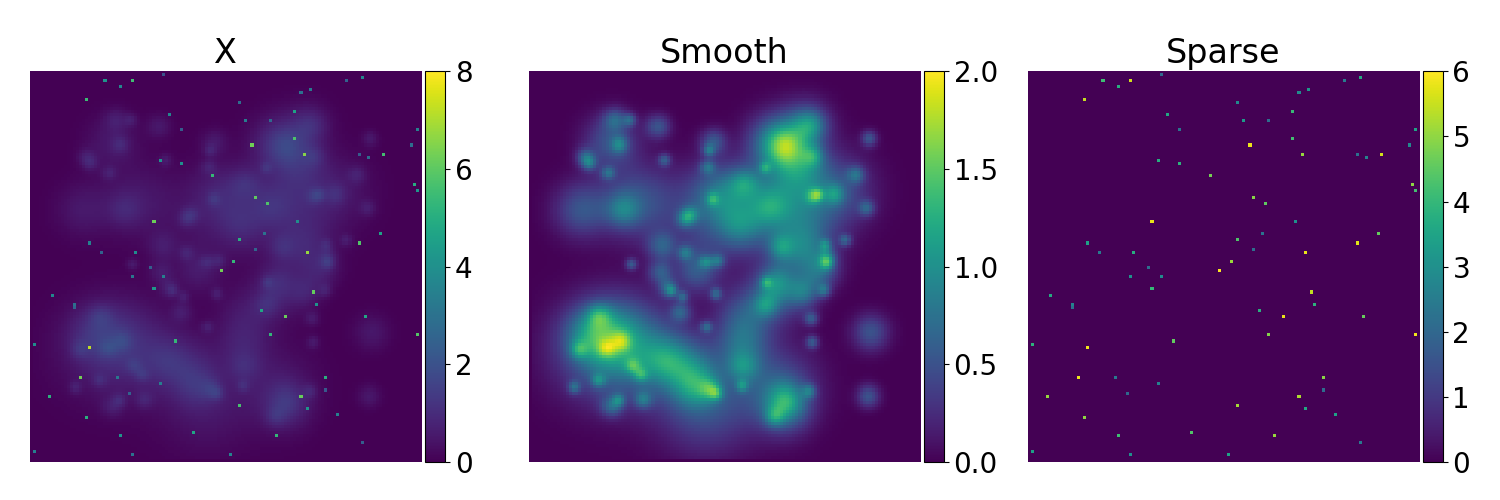
\includegraphics[width=1\textwidth]{SpareSmoothSignal.png}
    \caption{Sparse and smooth signal used to test the framework}
    \label{fig:SpareSmoothSignal}
\end{figure}

\section{Simulation and visualisation}
The last part we have to do is for testing our solver and visualise our images. To do this we create two files,  \verb+hyperparameter_testing.py+ for testing the solver on simulated signals, and \verb+util.py+ which contains plotting and metric functions. In the first file we have put all code used for the experiments of Chapter \ref{Results}. In \verb+util.py+ we put the plotting function used by \verb+hyperparameter_testing.py+, these plots are done with the package \verb+matplotlib+ with the function \verb+imshow()+. We also have some useful metrics functions that permits us to compare the reconstructions and the original.

\chapter{Results} \label{Results}
In this section we look at the performance of the framework. We will see how this composite model performs and compare it with two other more non-composite models, i.e. Lasso and Tikhonov. We will analyse the hyperparameters and see how they impact the reconstruction.

\subsection{Experimental setup}
All experiments are done with the following parameters except if explicitly told.
\begin{itemize}
    \item The original image is $128 \times 128$ pixels from Figure \ref{fig:SpareSmoothSignal}
    \item  We subsample 10 \% of the image's pixels with ”Gaussian + Uniform” sampling, from Figure \ref{fig:samp} (d).
    \item $\lambda_1$ and $\lambda_2$ are multiplied by $||H^*y||_{\infty}$ to scale with the image
    \item $\lambda_1 = 0.02$ ($\lambda_1$ = 0.02$||H^*y||_{\infty}$) and $\lambda_2 = 0.06$ ($\lambda_2$ = 0.06$||H^*y||_{\infty}$)
    \item PSNR of 50 (almost noiseless)
    \item The discrete Laplacian is used in the L2 penalty term
\end{itemize}

\section{Looking at a simple reconstruction}

\begin{figure}
    \centering
    \makebox[\linewidth]{
        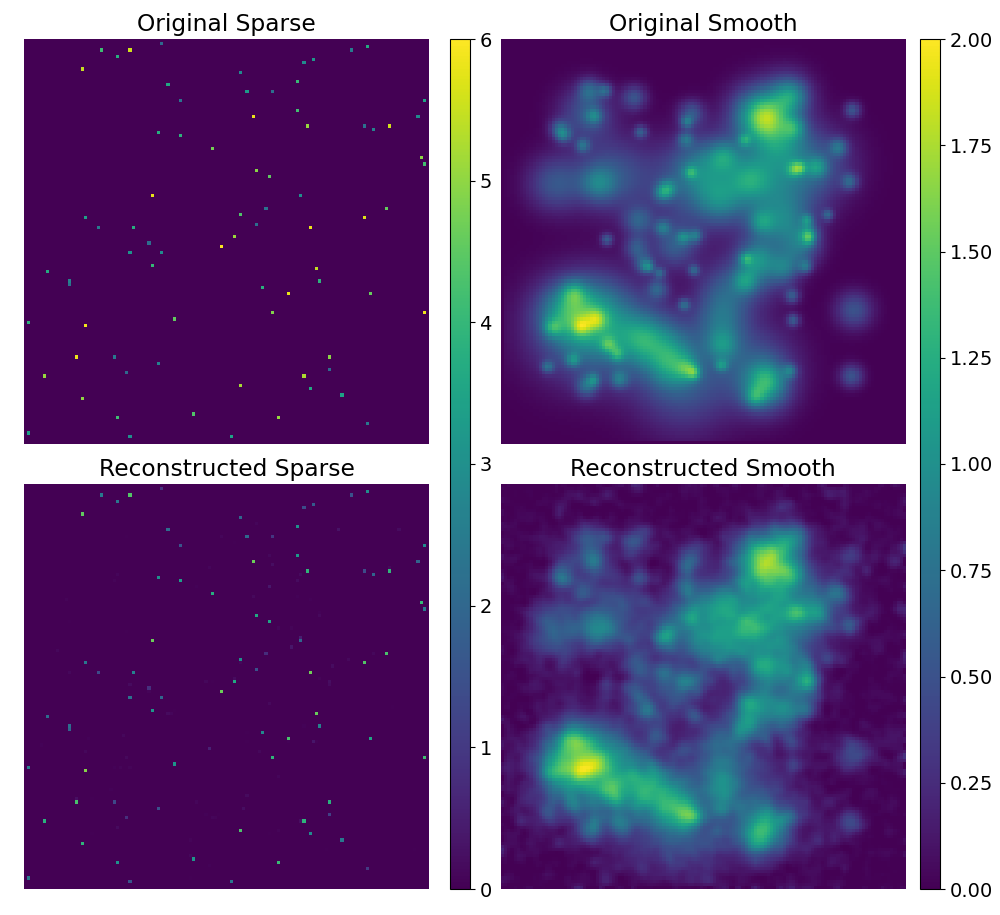
\includegraphics[width=1.5\textwidth]{SimpleReconstruction.png}}
    \caption{Reconstruction of a sparse and smooth image}
    \label{fig:SimpleReconstruction}
\end{figure}

\begin{figure}
    \centering
    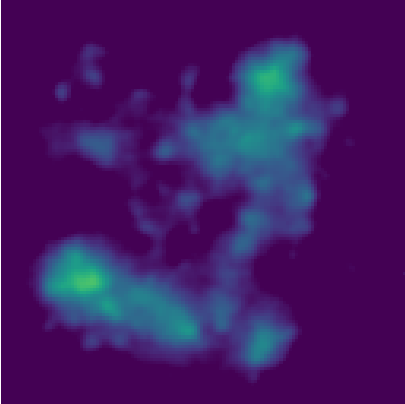
\includegraphics[width=0.4\textwidth]{Without positive constrain.png}
    \caption{Reconstruction without the positive constrain}
    \label{fig:Without positive constrain}
\end{figure}
We now look at a simple noiseless reconstruction. We plotted it in Figure \ref{fig:SimpleReconstruction}. We can see that the reconstruction work really well, we can recover each component and separate both as intended. The other noticeable thing is that here we only need to sample 10 \% of the image to have a precise reconstruction. We can recover all the peaks of the sparse component, but we lose energy due to the regularisation term on $x_1$ being a L1 norm and not a L0 norm which would be perfect but is not convex. For the smooth component, we see that the Laplacian does a good job at smoothing the reconstruction. The positive constrain makes our solution positive, to better see the effect we plotted the smooth reconstruction without the positive constrain on Figure \ref{fig:Without positive constrain} with the same scale between 0 and 2, we see that half of the signal is negative, thus is 0 on the plot. In contrary to the sparse component the smooth one doesn't lose energy in the reconstruction due to the positive constrain.

A small note on the performance of the algorithm, the reconstruction takes around 20 seconds on a desktop computer. For more realist size of $1000 \times 1000$ pixels, the time it takes is around 5 minutes. The performance is not the main focus of the project so we only talk briefly about it. The point is that even though we didn't focus on performance just using APGD with a fast operator suffice to have a solver that perform relatively well and can work on real world images.

\section{Measurement methods comparison}

In section \ref{methods} we talk about different methods of measurements, we will now look at how these impact the reconstruction. We have plotted the reconstruction done with each method in Figure \ref{fig:MeasurementMethodsReconstruction}. We first clearly see that if we want to recover a good smooth component using a uniform sampling does not work, as previously stated the smooth component is sparse in frequency concentrated in the low frequency around 0. So with the uniform sampling we only get very few of these coefficient and thus we can not reconstruct the smooth component. For the sparse component all methods can recover it perfectly, the only difference is their energy. If we look at the mean intensity of the reconstructions we have that the "uniform" has 92 \% of the original values and "Gaussian + Uniform" has only 70 \%.Which is quite a difference and is explained by the fact that the Fourier transform of the sparse image is spread in frequency so the "uniform" measure it better. The last interesting point is that the reconstruction with our "Gaussian + Uniform" method is almost as good the best sampling method, which justify even more the use of this method.

\begin{figure}
    \centering
    \makebox[\linewidth]{
        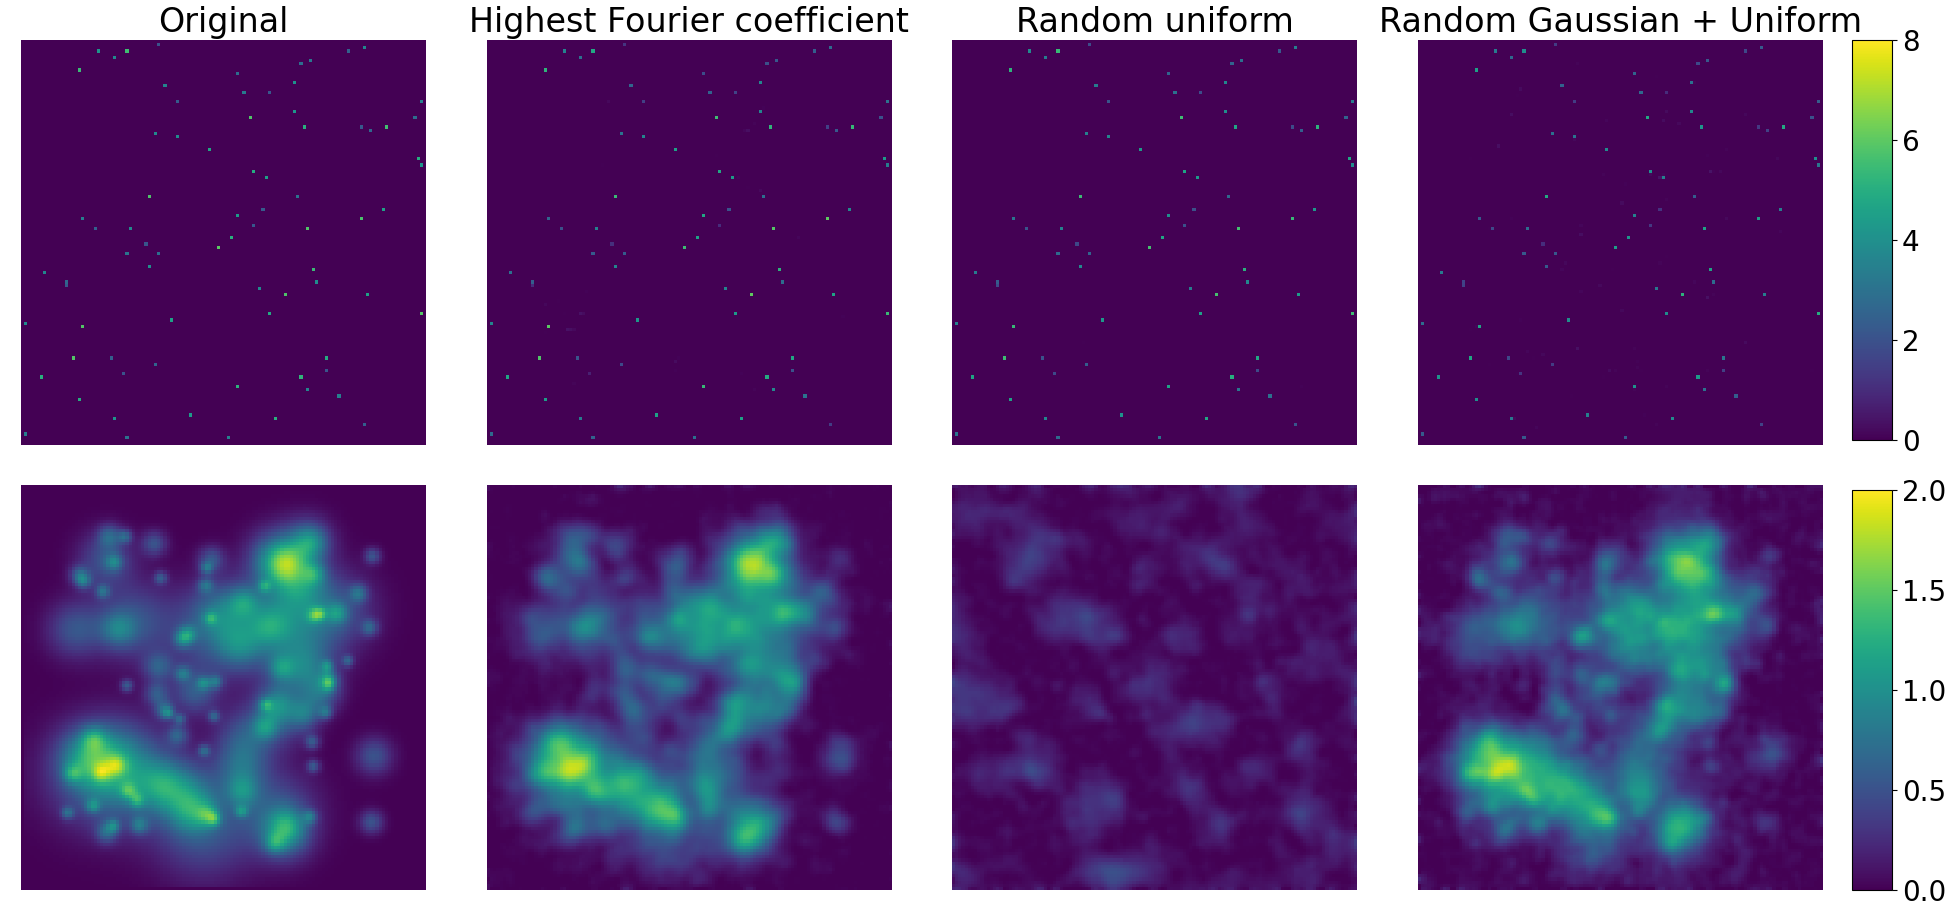
\includegraphics[width=1.5\textwidth]{MeasurementMethodsReconstruction.png}}
    \caption{Comparison of the measurement methods}
    \label{fig:MeasurementMethodsReconstruction}
\end{figure}


\section{Comparison with other models}

\begin{figure}
    \centering
    \makebox[\linewidth]{
        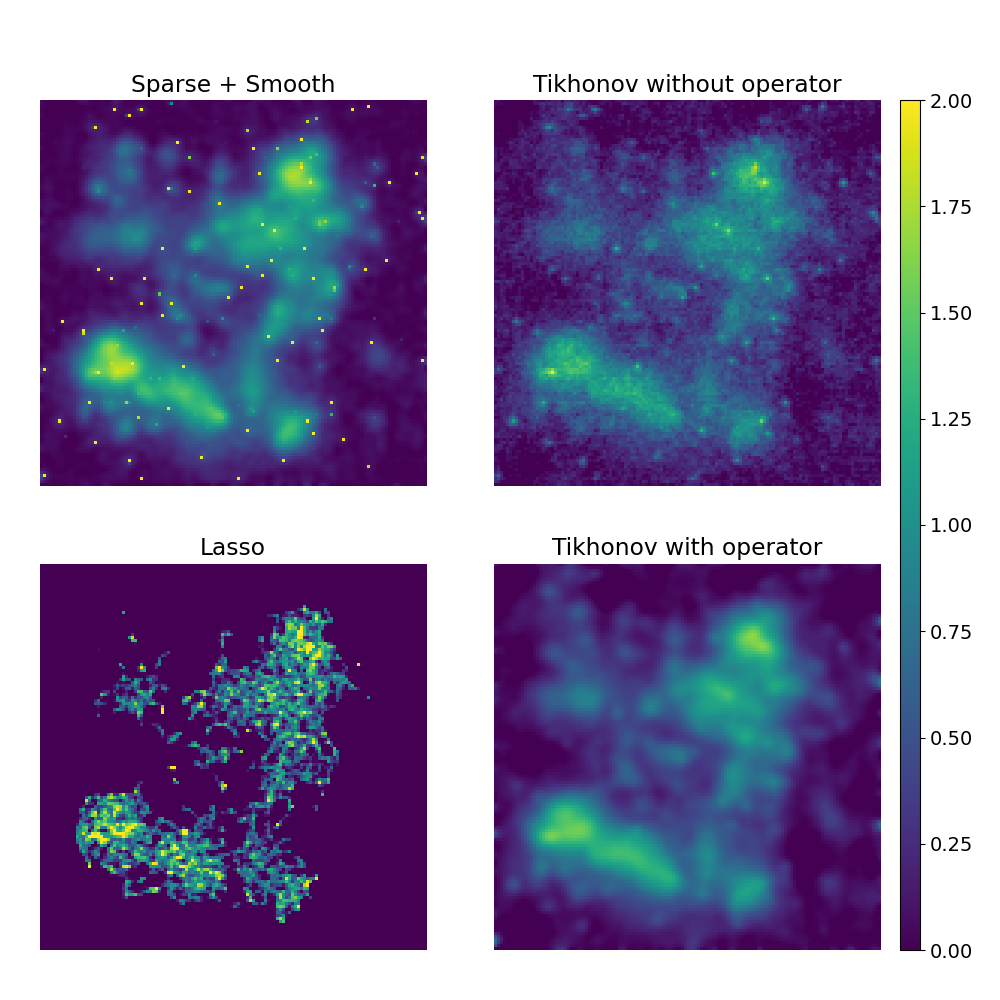
\includegraphics[width=1.5\textwidth]{comparison.png}}
    \caption{Comparison between solvers}
    \label{fig:comparison}
\end{figure}

We will now see how our model compares to Lasso and Tikhonov model. We have plotted the reconstructions done with each model in Figure \ref{fig:comparison} on the range 0 to 2 and not the full signal's range. We first have on top-left reconstruction done on Figure \ref{fig:SimpleReconstruction} where the yellow pixel are the spares component. On bottom-left we have the reconstruction done by the Lasso solver, the worse of all we can just recover vaguely the form of the smooth component. An import note is that the Lasso solver does not recover the sparse component, we could believe that since the image as a sparse component the Lasso solver could maybe reconstruct the sparse component only. This bad result is not really surprising since the Representer Theorem I tells us that we can recover only 10\% of the image, so we can never recover the original image completely. As for Tikhonov, we have two models, one where we use the Laplacian and the other without. First we see that this model is already much better than Lasso and much more accurate. Especially on the bottom-right with a smoothing operator the reconstruction is almost as good as the smooth one from our model. On top-right without Laplacian is also good in terms of precision to the smooth component, but without this smooth property. The problem with Tikhonov's model is with the sparse component, if we use a smoothing operator then the sparse component completely disappear from the reconstruction. Even without it, we can only get a bit of the sparse component. So with Tikhonov we need to choose between the smoothness and the sparsity, we can not have both. Even if the want sparsity it remains difficult to get a clean sparse component as in our model, and the energy of it becomes very low since we minimize the L2 norm. Another important point is that using these models we can only reconstruct $\boldsymbol{x}$ and we can not have the two component separated as we have with our model.

\section{Smoothing operator}

\begin{figure}
    \centering
    \makebox[\linewidth]{
        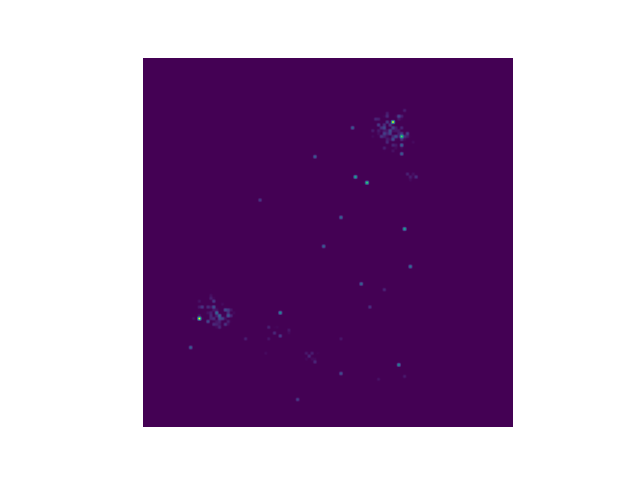
\includegraphics[width=0.57\textwidth]{sparse_without_smooth.png}}
    \caption{Reconstructed sparse component without smoothing operator}
    \label{fig:sparse_without_smooth}
\end{figure}

\begin{figure}
    \centering
    \makebox[\linewidth]{
        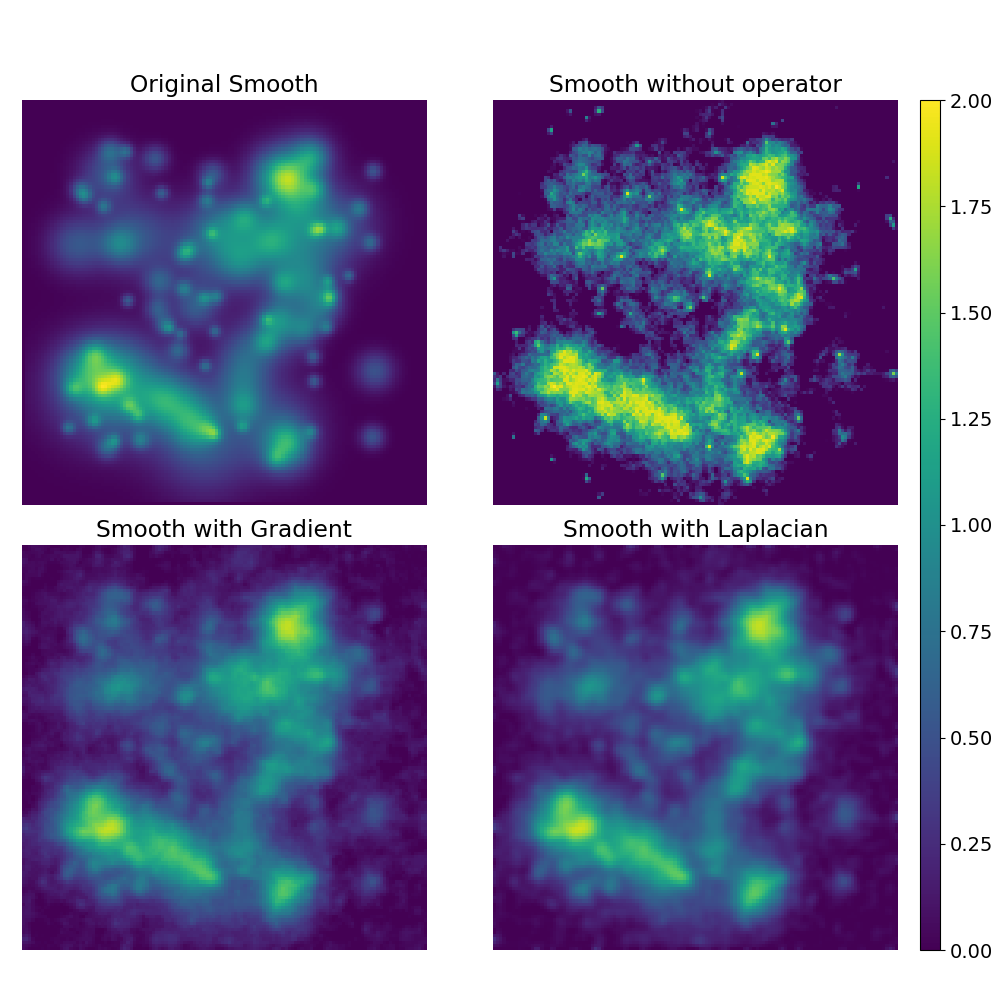
\includegraphics[width=1.5\textwidth]{smoothing.png}}
    \caption{Comparison of the smoothing operator}
    \label{fig:smoothing}
\end{figure}

In this section we will see how the smoothing operator impacts the reconstruction. We have plotted the smooth reconstructions in Figure \ref{fig:smoothing} done with the Gradient, Laplacian and without operator. First we can see that the choice of the smoothing operator is not that important we have not much difference between Gradient and Laplacian. The only different is that the low values spread less and go to 0 more quickly. When we look at the reconstruction without operator, we see a non-smooth reconstruct that is much worse that the reconstruction done by Tikhonov. We see some peaks of the sparse component that pollute the smooth one. It also breaks the sparse reconstruction as shown in Figure \ref{fig:sparse_without_smooth}. So the smoothing operator has two effect, first it smooth the result as wanted and second it eliminates the sparse peaks of the smooth reconstruction.

\section{Tuning parameters $\lambda_1$ and $\lambda_2$} \label{Tuning parameters}

\begin{figure}
\begin{center}
\begin{tabular}{||c c c||}
 \hline
 $lambda_1$ & $lambda_2$ & Wasserstein dist\\ [0.5ex]
 \hline\hline
 0.02 & 0.02 & 7.19e-06\\
 0.02 & 0.06 & 9.68e-06 \\
 0.06 & 0.15 & 1.16e-05 \\
 0.06 & 0.06 & 1.38e-05 \\
 0.06 & 0.30 & 1.52-05 \\
 0.06 & 0.02 & 2.51e-05 \\
 0.15 & 0.30 & 2.81e-05 \\
 0.15 & 0.15 & 3.64e-05 \\
 0.02 & 0.15 & 4.17e-05 \\
 0.15 & 0.06 & 5.18e-05 \\
 0.02 & 0.30 & 9.14e-05 \\
 0.30 & 0.30 & 9.39e-05 \\
 0.30 & 0.06 & 9.67e-05 \\
 0.30 & 0.02 & 0.0049 \\
 0.30 & 0.15 & 0.0021 \\
 0.15 & 0.02 & 0.0069 \\
 [1ex]
 \hline
 \end{tabular}
 \hfil  
 \begin{tabular}{||c c c||}
 \hline
 $lambda_1$ & $lambda_2$ & NMSE\\ [0.5ex]
  \hline\hline
 0.02  & 0.06 & 0.009 \\
 0.02  & 0.15 & 0.010 \\
 0.06  & 0.30 & 0.011 \\
 0.06  & 0.15 & 0.011 \\
 0.02  & 0.02 & 0.012 \\
 0.06  & 0.06 & 0.014 \\
 0.15  & 0.30 & 0.015 \\
 0.15  & 0.15 & 0.016 \\
 0.30  & 0.30 & 0.018 \\
 0.30  & 0.15 & 0.021 \\
 0.15  & 0.06 & 0.024 \\
 0.06  & 0.02 & 0.026 \\
 0.30  & 0.06 & 0.030 \\
 0.02  & 0.30 & 0.039 \\
 0.30  & 0.02 & 0.048 \\
 0.15  & 0.02 & 0.049 \\
 [1ex]
 \hline
 \end{tabular}
\end{center}
    \caption{Loss of each component to the original image for different $\lambda$ sorted from smallest to highest}
    \label{lambda table}
\end{figure}

\begin{figure}
    \centering
    \makebox[\linewidth]{
        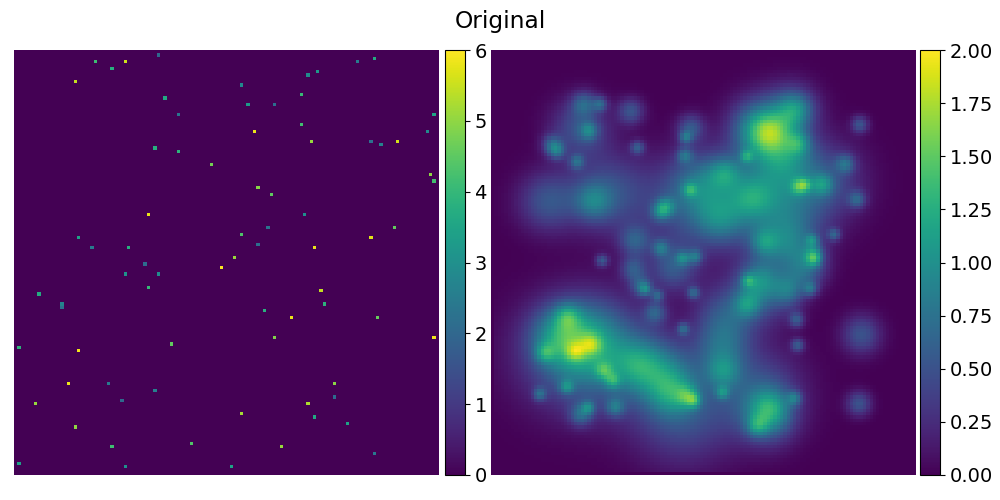
\includegraphics[width=0.85\textwidth]{Original.png}}
    \makebox[\linewidth]{
        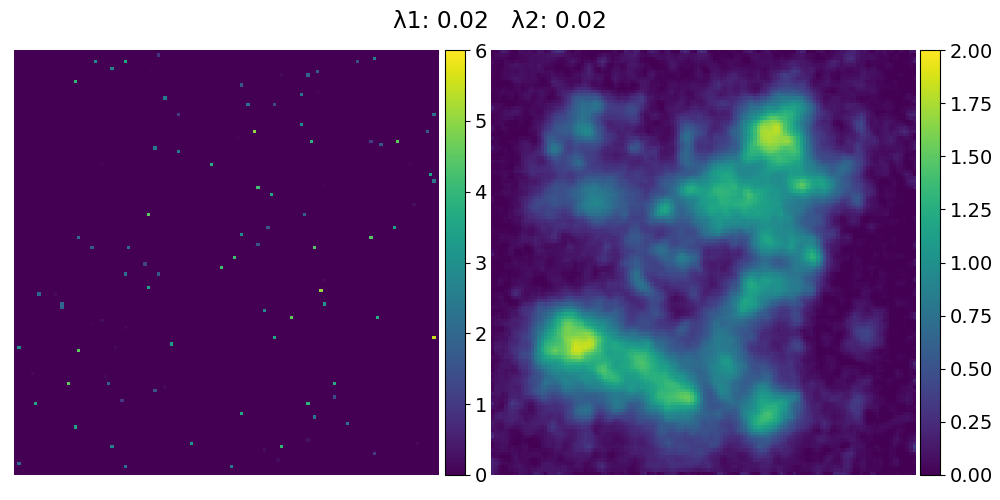
\includegraphics[width=0.85\textwidth]{λ102λ202.png}}
    \makebox[\linewidth]{
        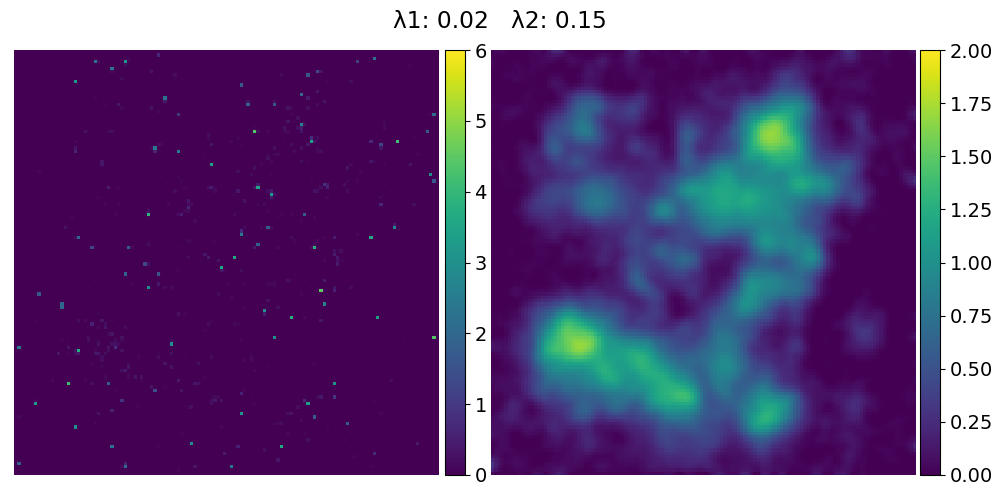
\includegraphics[width=0.85\textwidth]{λ102λ215.png}}
    \makebox[\linewidth]{
        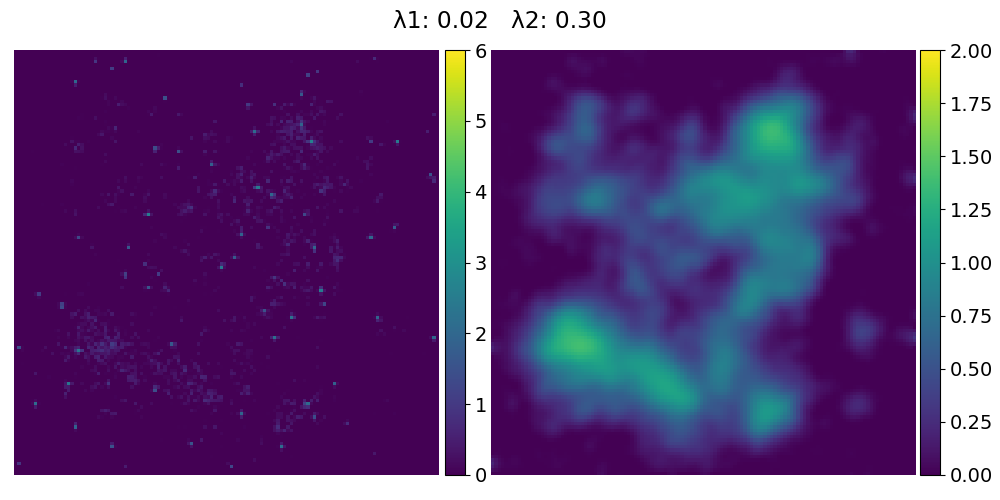
\includegraphics[width=0.85\textwidth]{λ102λ230.png}}
    \caption{Reconstructions with different $\lambda$}
    \label{fig:lambdas}
\end{figure}

\begin{figure}
    \centering
    \ContinuedFloat
   \makebox[\linewidth]{
        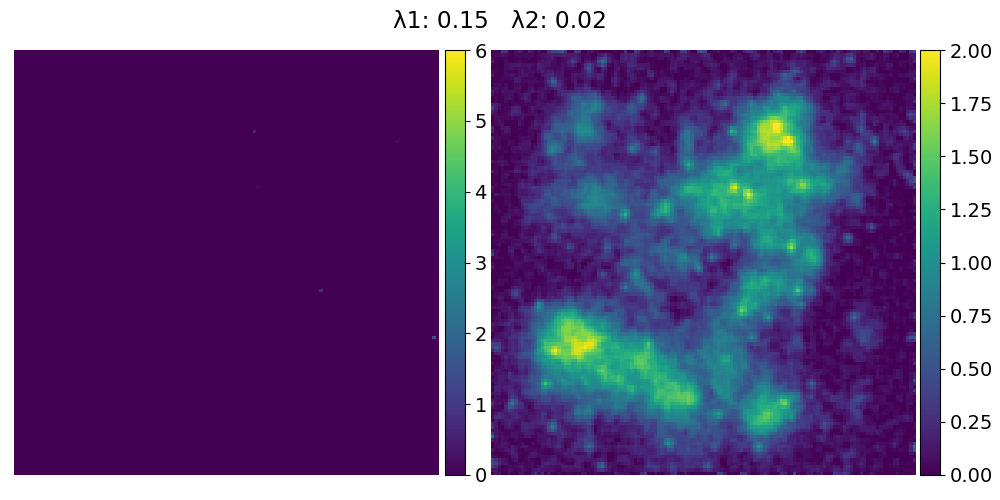
\includegraphics[width=0.85\textwidth]{λ115λ202.png}}
    \makebox[\linewidth]{
        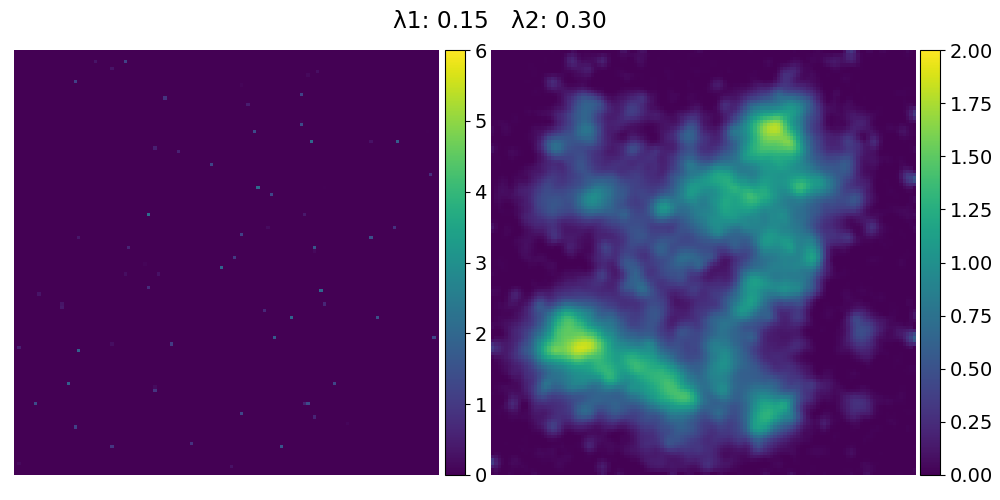
\includegraphics[width=0.85\textwidth]{λ115λ230.png}}
    \makebox[\linewidth]{
        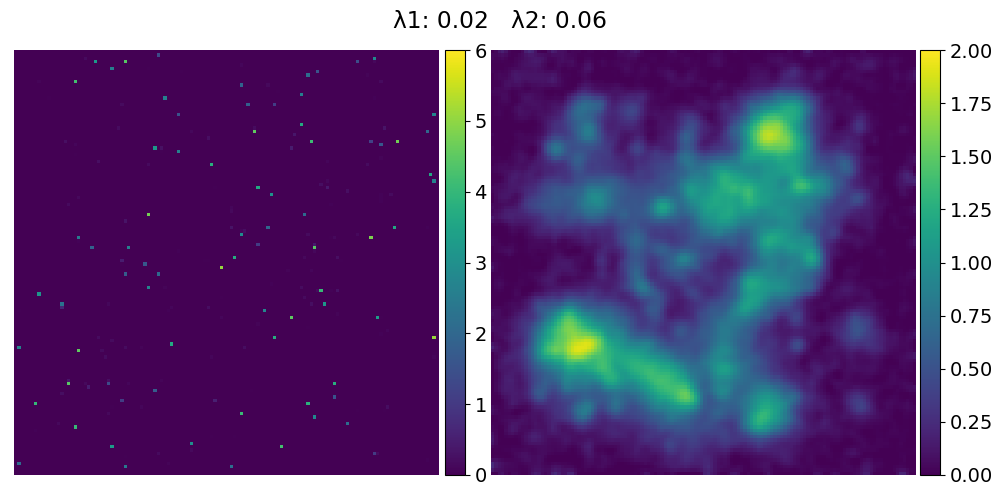
\includegraphics[width=0.85\textwidth]{λ102λ206.png}}
    \makebox[\linewidth]{
        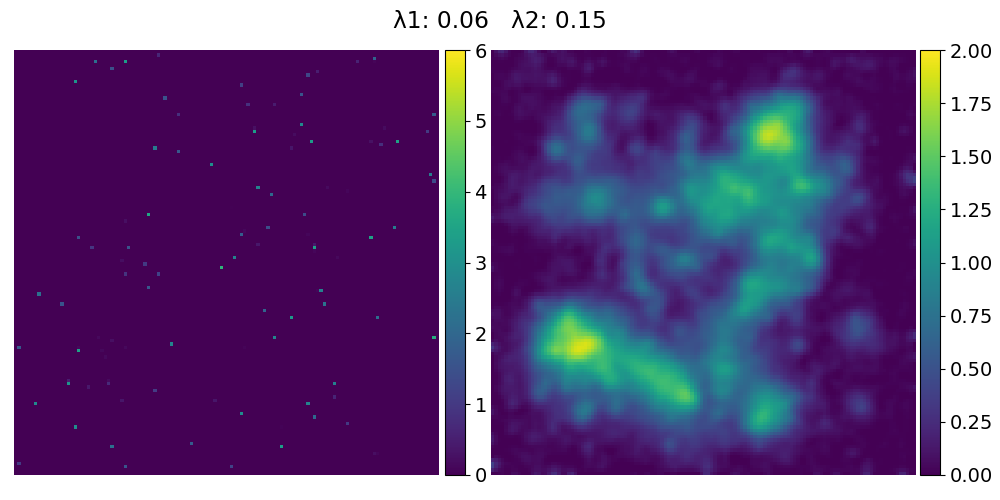
\includegraphics[width=0.85\textwidth]{λ106λ215.png}}
    \caption{Reconstructions with different $\lambda$}
\end{figure}

\begin{figure}
    \centering
    \makebox[\linewidth]{
        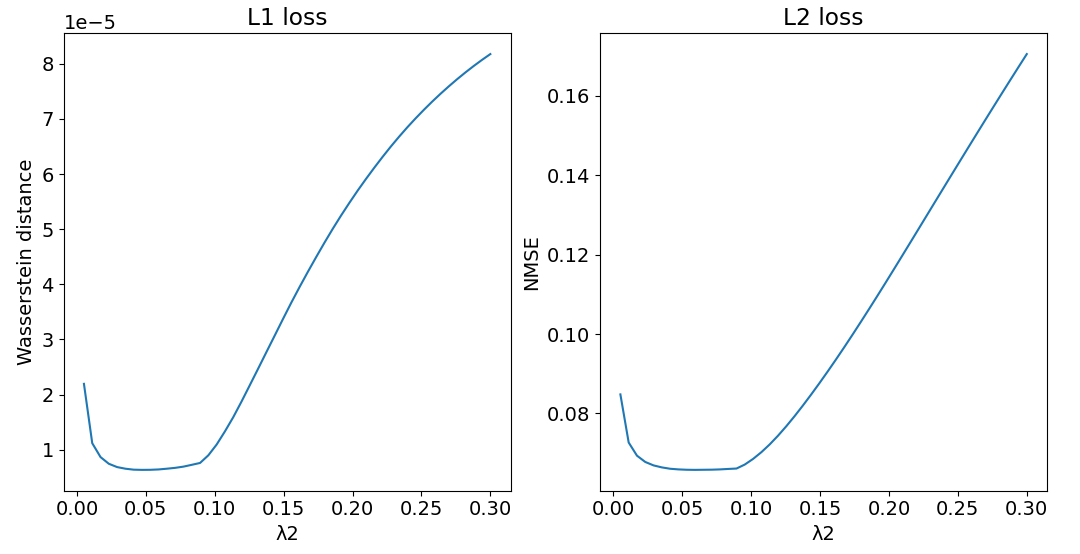
\includegraphics[width=1.1\textwidth]{Loss_comparisonl2.png}}
    \caption{Loss comparison where we fix $\lambda_1 = 0.02$ and change $\lambda_2$}
    \label{fig:lossl2}
\end{figure}

\begin{figure}
    \centering
    \makebox[\linewidth]{
        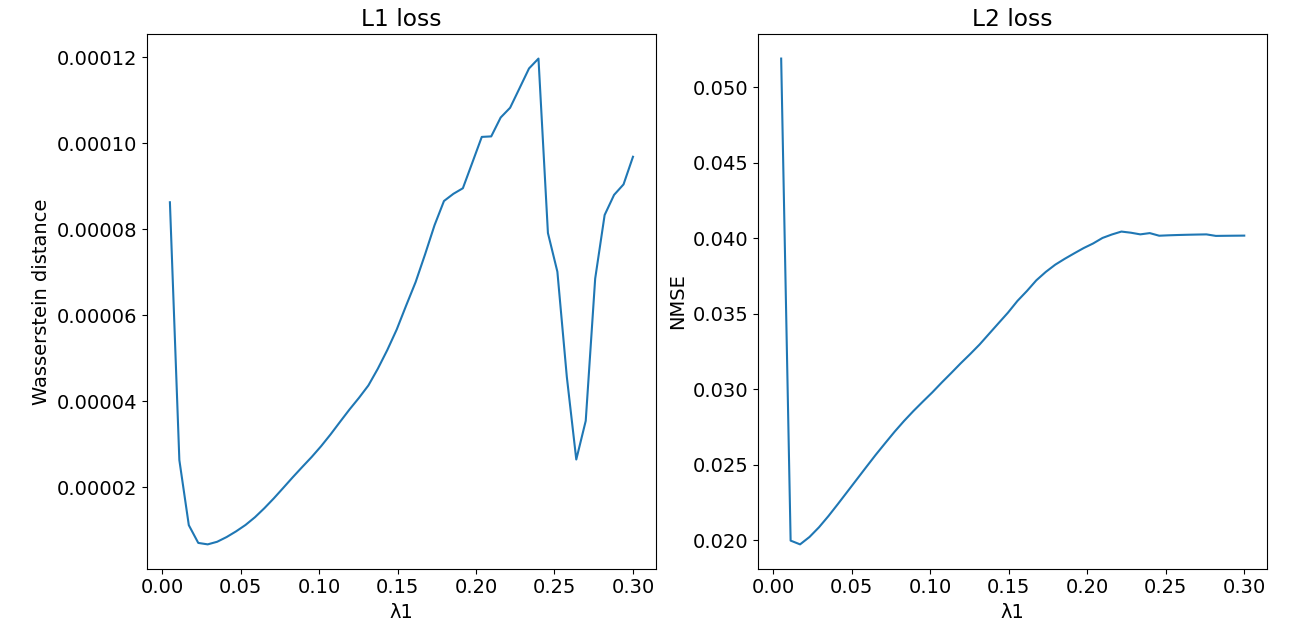
\includegraphics[width=1.15\textwidth]{Loss_comparisonl1.png}}
    \caption{Loss comparison where we fix $\lambda_2 = 0.06$ and change $\lambda_1$}
    \label{fig:lossl1}
\end{figure}

We will now see the impact of the tuning parameters on the reconstruction. To see this we have plotted on Figure \ref{fig:lambdas} reconstructions with different $\lambda$, $0.02$, $0.06$, $0.15$ and $0.3$ and on Figure \ref{lambda table} we have the loss of each reconstructed component with the original. On Figure \ref{fig:lambdas}, first we try to augment $\lambda_2$  for a given $\lambda_1$, we see that as $\lambda_2$ increase the smooth reconstruction has less energy, to the point where at $\lambda_2 = 0.3$ we start to lose a lot of precision on the data fidelity. As for the sparse component, it becomes more permissive and starts to have some noisy values. Then we augment $\lambda_1$ to 0.15, we see that the reconstruction depends on $\lambda_2$, with a small one we got a almost zero sparse component with a very noisy smooth one, and with a bigger $\lambda_2$ we got a better reconstruction, but not as good as with a smaller $\lambda_1$. So we can conclude that $\lambda_1$ seems to need to be the smallest possible, but not too small as for the solver to not explode. Also with too small $\lambda_1$ compare to $\lambda_2$, we start to get noisy values in the sparse component. It seem like $\lambda_1 = 0.02$ is a good value. We can confirm that with Figure \ref{lambda table} where we see that the smallest loss for both component is when $\lambda_1 = 0.02$. 

As for finding the best value for $\lambda_2$ it depends on $\lambda_1$, as said increasing $\lambda_2$ makes the smooth component to have less energy, but with a bigger $\lambda_1$ the energy augments. We can see this effect we comparing the image 4th and 6th image with $\lambda_2 = 0.3$ where in the second one we have a better smooth reconstruction. And so it seems that $\lambda_2$ need to be proportional to $\lambda_1$, our finding is that $\lambda_2$ should be around 2 to 6 times $\lambda_1$, and in the worse case at least $\lambda_2 = \lambda_1$ and a maximum of around 10 times. We can confirm this by looking at Figure \ref{lambda table} where all images with the least NMSE have this proportionality, and at the end we have those that have a too big difference or where $\lambda_2 < \lambda_1$. But this does seem to be the case for $\lambda_1$, we just need a difference ratio that is not too big.

To resume, to choose the tuning parameters, we first choose $\lambda_1$ with $\lambda_1 = \lambda_2$ to have a good sparse reconstruction and then we take $\lambda_2$ to be 1 to 6 times the chosen $\lambda_1$. We adjust these depending on the desired reconstruction, lower $\lambda_2$ to have a sparser $\boldsymbol{x}_1$ and higher $\lambda_2$ to have more pixels in $x_1$. To confirm these values we can do more tests, on Figure \ref{fig:lossl2} and \ref{fig:lossl1} we have plot the loss of each component when changing each $\lambda$ with the other one fixed. On Figure \ref{fig:lossl2} we can clearly see that when we fix $\lambda_1 = 0.02$ then we can only vary $\lambda_2$ from $\lambda_2 = \lambda_1$ to $\lambda_2 = 6 \lambda_1$ for an optimal loss. On Figure \ref{fig:lossl1}, we see that when varying $\lambda_1$ we have an optimal value $\lambda_1 = 0.03$ that appears.

\section{Noise}

\begin{figure}
    \centering
    \makebox[\linewidth]{
        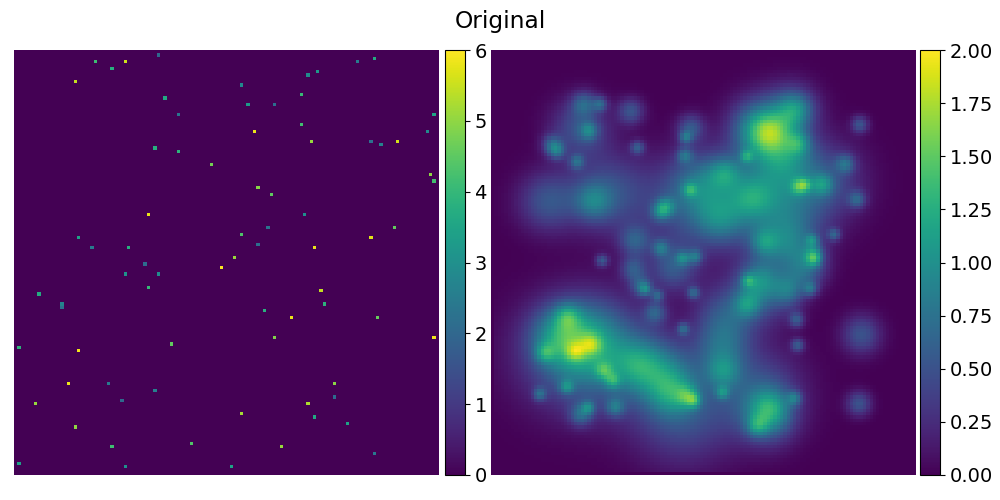
\includegraphics[width=0.85\textwidth]{Original.png}}
    \makebox[\linewidth]{
        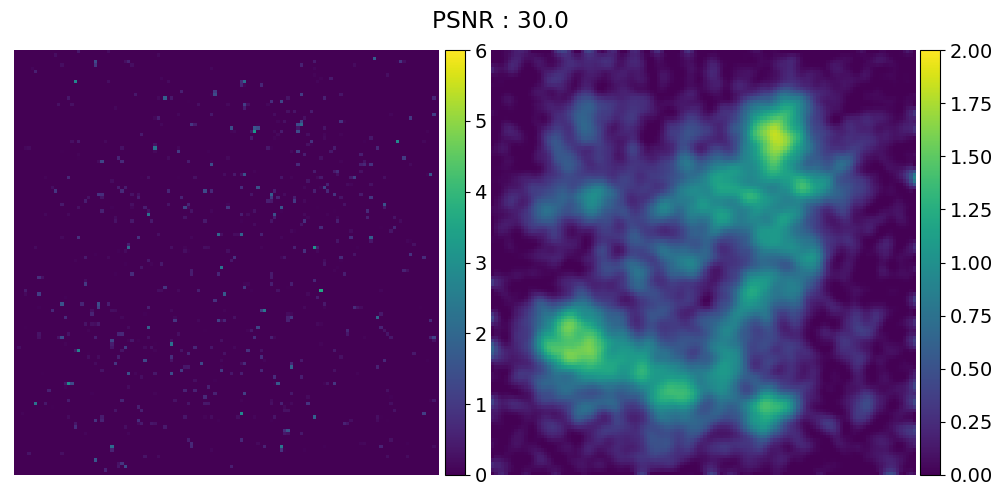
\includegraphics[width=0.85\textwidth]{PSNR30.png}}
    \makebox[\linewidth]{
        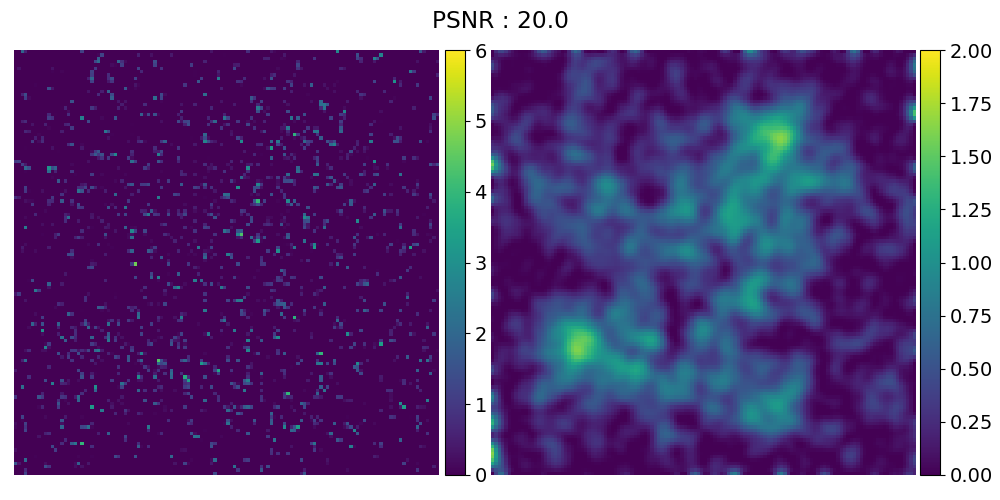
\includegraphics[width=0.85\textwidth]{PSNR20.png}}
    \makebox[\linewidth]{
        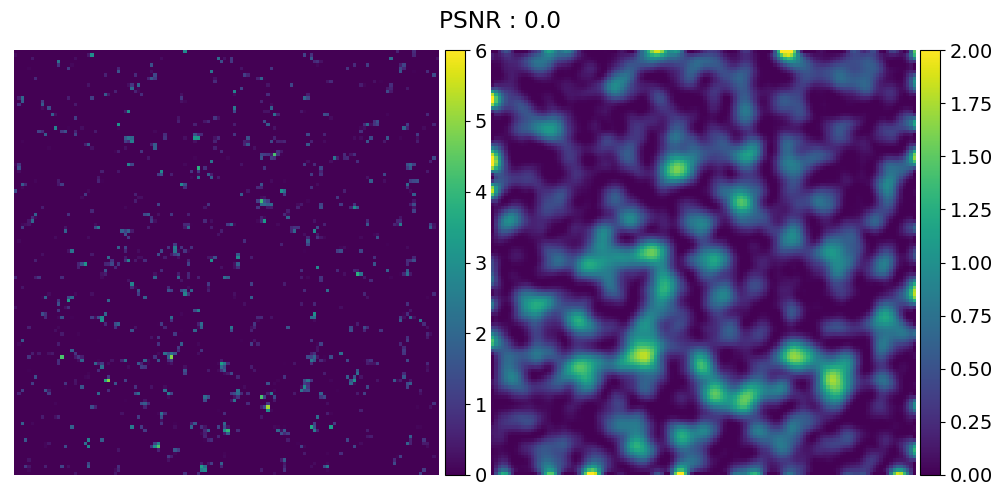
\includegraphics[width=0.85\textwidth]{PSNR0.png}}
    \caption{Reconstructions with different PSNR}
    \label{fig:noise}
\end{figure}

Until now we have seen the framework working on almost noiseless image (i.e. 50 PSNR), we will now see how the noise impact the reconstructions. To do so we first make some reconstruction with different level of noise on Figure \ref{fig:noise}, for each one we have adapted the intensity of the penalty. We see directly that with too much noise (i.e. 0 PSNR) we can not reconstruct anything. For the other values the smooth component it generally quite good and the quality depends directly on the the amount of noise. For the sparse reconstruct it is more complicated, generally we can only recover the high energy values. The low energy values can not be recovered due to noisy peaks appearing, can we see this effect on Figure \ref{fig:20 sparse} where we have taken some pixels of the sparse component and see how their values changes when $\lambda_1$ change for a fixed $\lambda_2 = 0.6$ at 20 PSNR. We have classified the pixel in two group, in blue the originals values that should be recover and the ones that should to zeros in orange. In this plot we see that as $\lambda_1$ increase the image become sparser, also the more energy one pixel has the longer he can last. So to eliminate the noisy values we need a high $\lambda_1$, here $\lambda_1$ would be around 0.4, but such high $\lambda_1$ also eliminate a lot of low energy pixel from the reconstruct. So the sparse reconstruction can only be partial, we can recover only the highest energy values, and this number depends on the amount of noise.

For noisy measurements what we can reconstruct depends strongly on the value on the tuning parameters $\lambda_1$ and $\lambda_2$. To analyse them we have done the same loss plot as in section \ref{Tuning parameters}. When we look at the loss plot on Figure \ref{fig:20 lossl1} we can find one minimum on each graph, for the first one, it happens when we have eliminate most of the noise and have only a few remaining peaks on the sparse component. For the second one we are on the point where we have the good ratio  $\lambda_2 = 4 \lambda_1$ as discussed on section \ref{Tuning parameters} and so the best data fidelity on $\boldsymbol{x}_2$, but with a worse $\boldsymbol{x}_1$. To confirm these conclusion we plot the reconstructions with the parameters given by the graph on Figure \ref{fig:20 lossl1 rec}. We can clearly see that on the first minimum we have indeed only a few non-zero values and for the second one we have a lot more noisy peaks on the sparse component with a bit better data fidelity on the smooth component since the energy is lessen. Then on Figure \ref{fig:20 lossl2} we find that to have a good smooth reconstruction we need to augment $\lambda_2$, but doing so makes us lose precision on the sparse one, because we have noisy values that appear. To confirm this we also plot the extreme case on Figure \ref{fig:20 lossl2 rec}, where we see that with a high $\lambda_2 = 1.1$ we have a better smooth component, but then we erase the sparse one and for a low $\lambda_2 = 0.2$ we worsen the smooth reconstruction, but have a better sparse. 



\begin{figure}
    \centering
    \makebox[\linewidth]{
        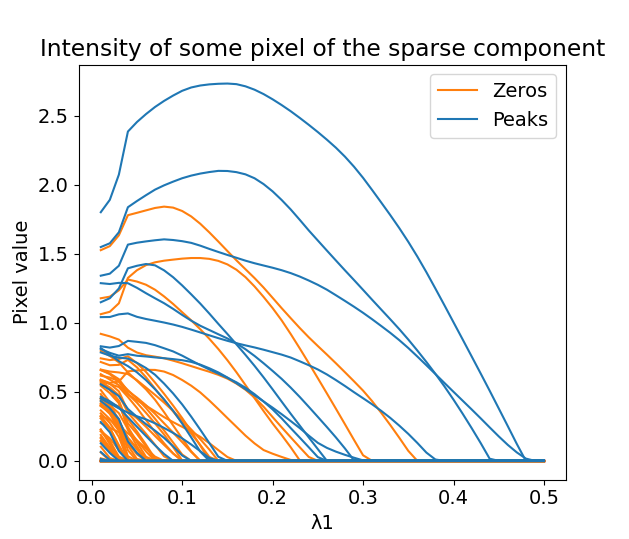
\includegraphics[width=0.9\textwidth]{Following_some_pixel_of_the_sparse_component.png}}
    \caption{Following some pixel of the sparse component, with 20 PSNR and $\lambda_2 = 0.6$}
    \label{fig:20 sparse}
\end{figure}

\begin{figure}
    \centering
    \makebox[\linewidth]{
        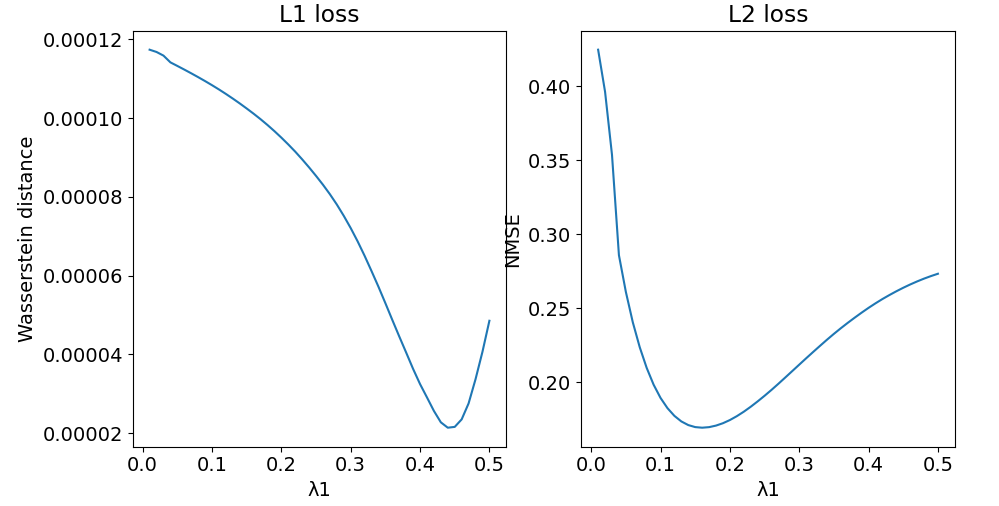
\includegraphics[width=1.2\textwidth]{Loss_comparison20l1.png}}
    \caption{Loss comparison where we fix $\lambda_2 = 0.6$ with 20 PSNR}
    \label{fig:20 lossl1}
\end{figure}

\begin{figure}
    \centering
    \makebox[\linewidth]{
        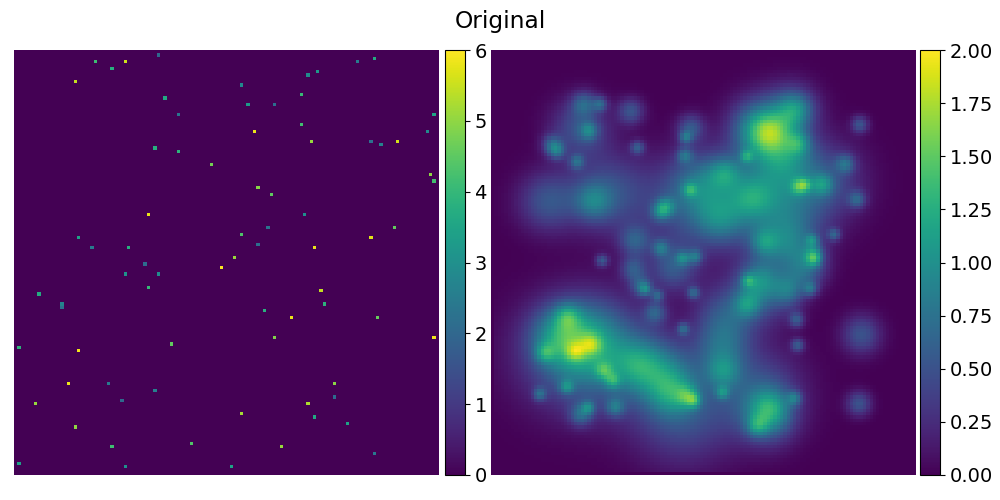
\includegraphics[width=1.1\textwidth]{Original.png}}
    \makebox[\linewidth]{
        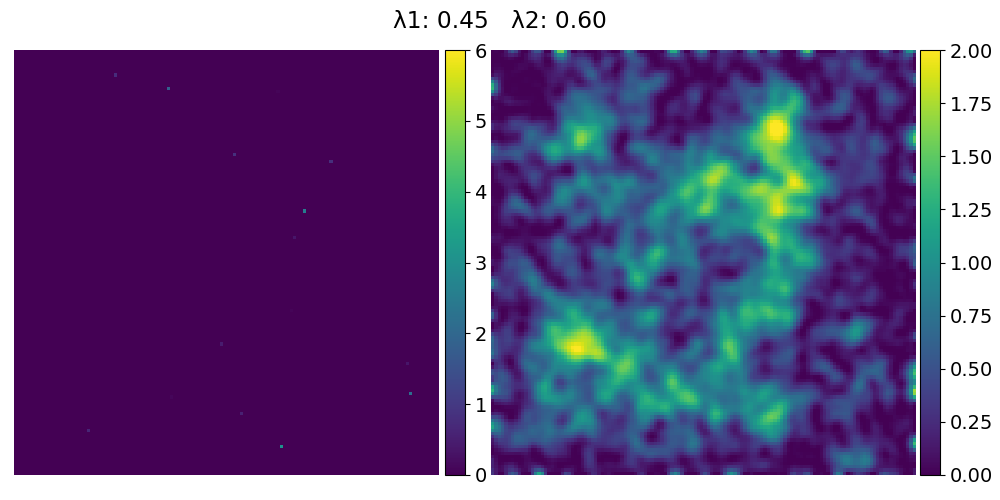
\includegraphics[width=1.1\textwidth]{λ145λ260.png}}
    \makebox[\linewidth]{
        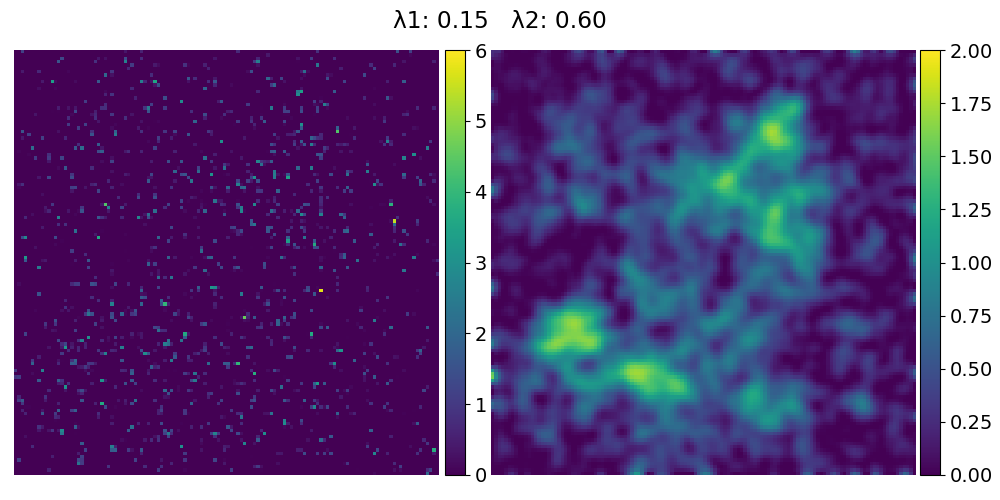
\includegraphics[width=1.1\textwidth]{λ115λ260.png}}
    \caption{Reconstruction where we fix $\lambda_1 = 0.25$ and see the impact of $\lambda_2$ with 20 PSNR}
    \label{fig:20 lossl1 rec}
\end{figure}

\begin{figure}
    \centering
    \makebox[\linewidth]{
        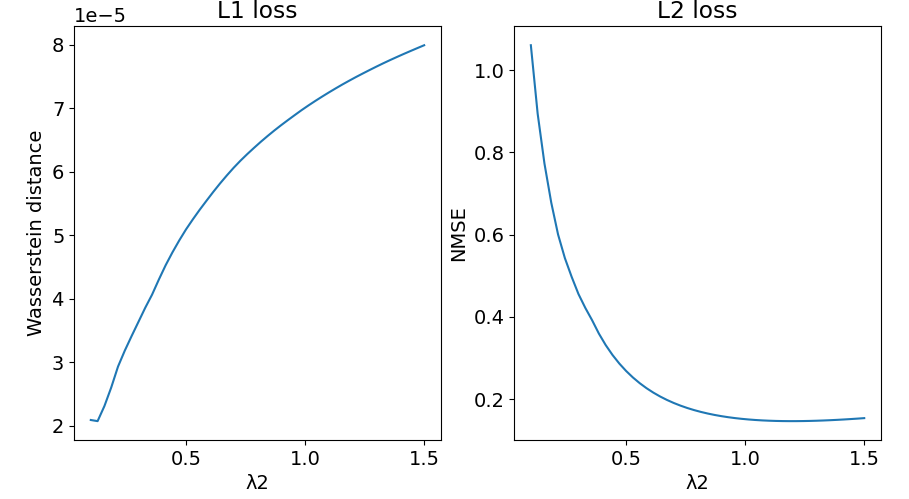
\includegraphics[width=1.2\textwidth]{Loss_comparison20l2.png}}
    \caption{Loss comparison where we fix $\lambda_1 = 0.25$ with 20 PSNR}
    \label{fig:20 lossl2}
\end{figure}

\begin{figure}
    \centering
    \makebox[\linewidth]{
        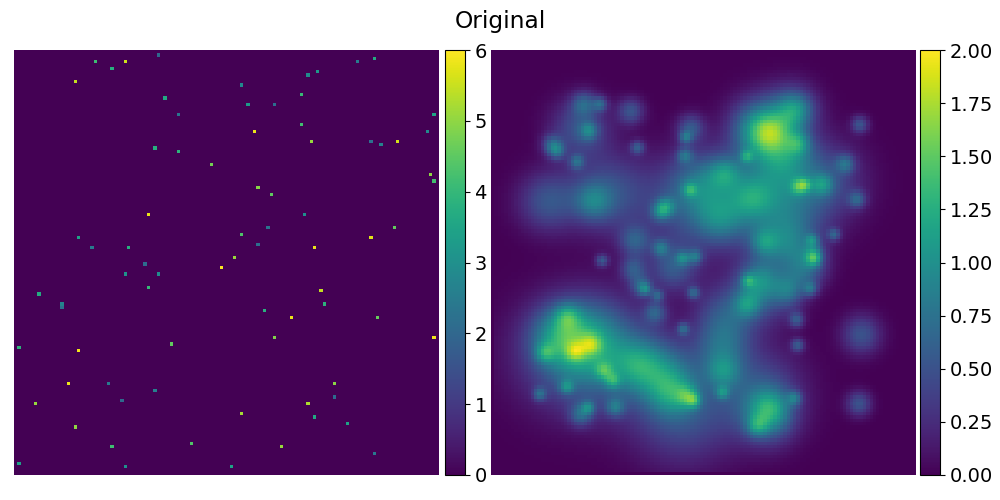
\includegraphics[width=1.1\textwidth]{Original.png}}
    \makebox[\linewidth]{
        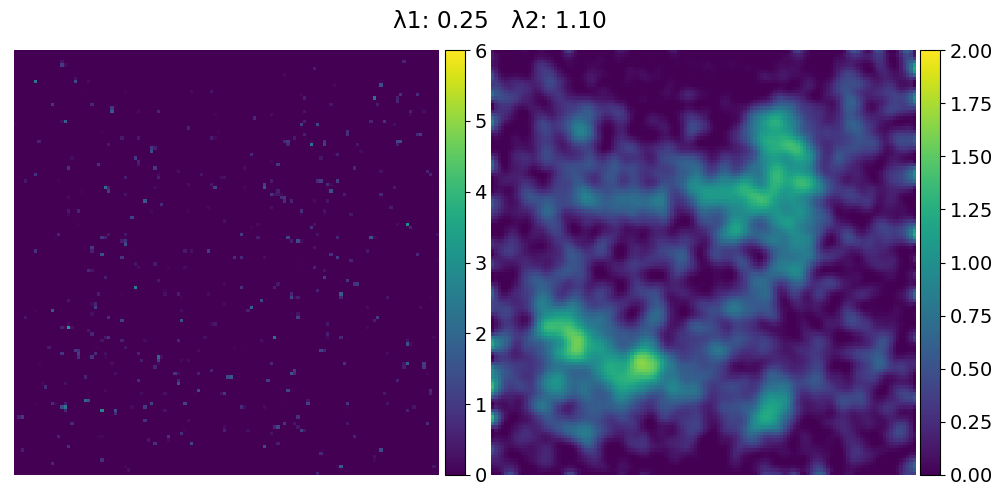
\includegraphics[width=1.1\textwidth]{λ125λ2110.png}}
    \makebox[\linewidth]{
        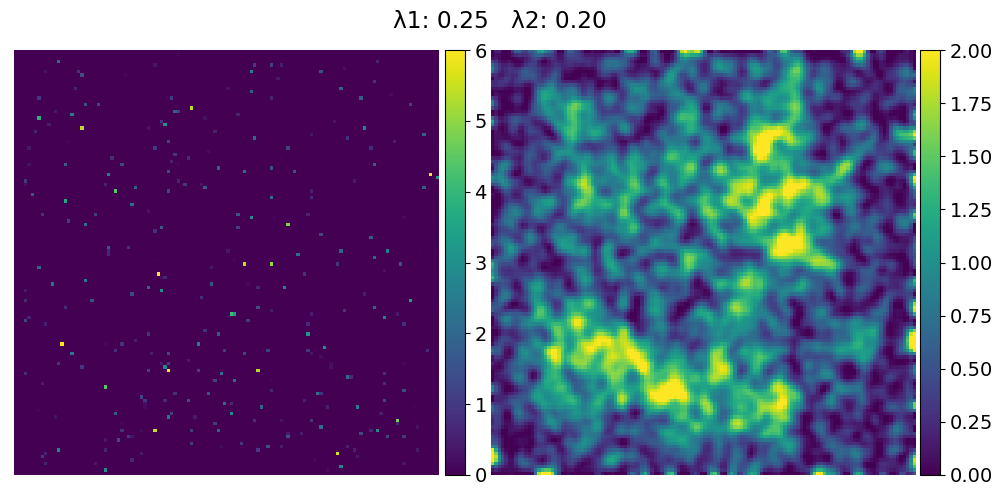
\includegraphics[width=1.1\textwidth]{λ125λ220.png}}
    \caption{Reconstruction where we fix $\lambda_1 = 0.25$ and see the impact of $\lambda_2$ with 20 PSNR}
    \label{fig:20 lossl2 rec}
\end{figure}

Putting both graph together we see that each $\lambda$ impact strongly it's own component, i.e. to eliminates the noisy peaks on the sparse component we need to increase $\lambda_1$ and to have a better smooth reconstruction we need to increase $\lambda_2$, but each $\lambda$ also has a smaller impact on the other component and so the reconstruction of each component depends also on the radio between $\lambda_1$ and $\lambda_2$. This join what we discover in section \ref{Tuning parameters}, where $\lambda_1$ and $\lambda_2$ needs to be proportional, it seems that with noise it is less the case, but has still some importance. We see with Figure \ref{fig:20 lossl1 rec} that for a given $\lambda_2$, $\lambda_1$ change the energy of the smooth reconstruction and on Figure \ref{fig:20 lossl2 rec} that for a given $\lambda_1$, $\lambda_2$ also change the energy of the sparse one. 

To conclude, with noisy measurement we not only need to find the right intensity of penalty to mitigate the noise, but also find the right ratio between $\lambda_1$ and $\lambda_2$ to have the desired precision on each component. 

\section{Real-world images}

\begin{figure}
    \centering
    \makebox[\linewidth]{
        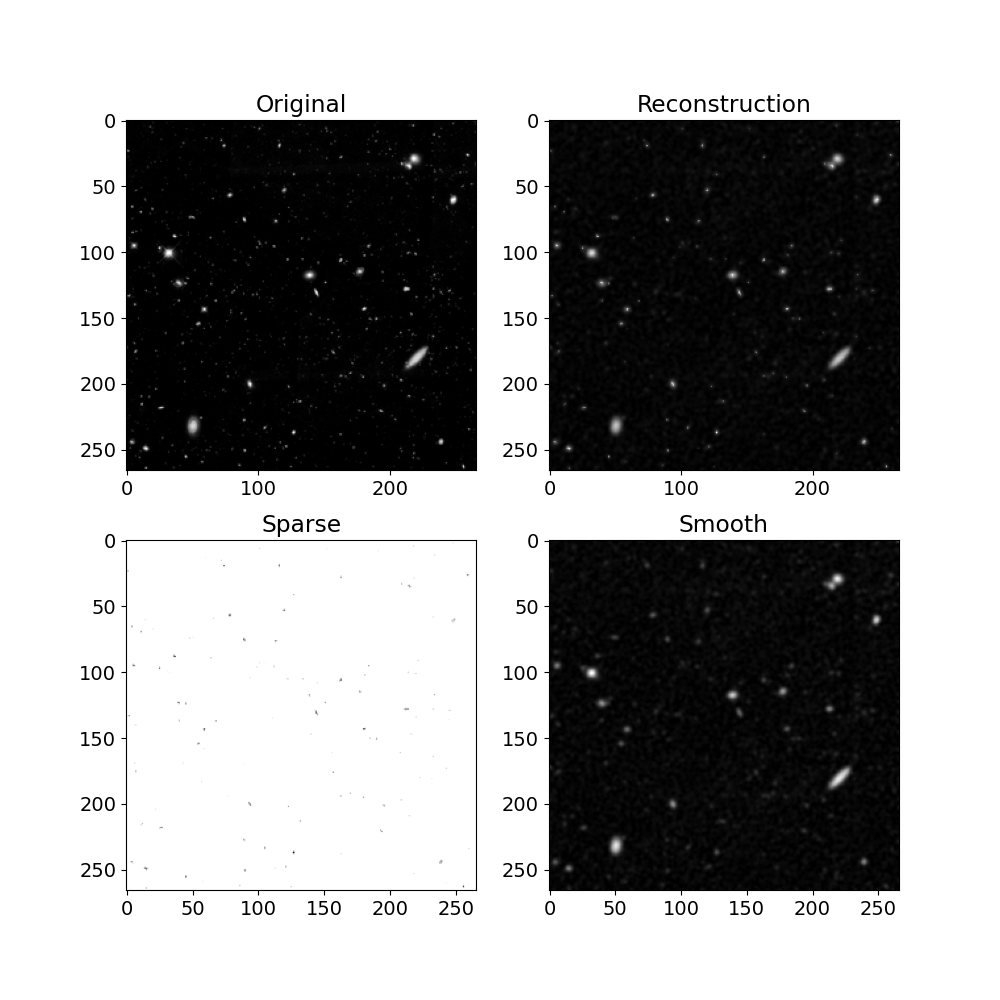
\includegraphics[width=1.7\textwidth]{h7.png}}
    \caption{Reconstruction of a real low dimensional image with $\lambda_1 = 0.02$ and $\lambda_2 = 0.06$}
    \label{fig:h7}
\end{figure}

\begin{figure}
    \centering
    \makebox[\linewidth]{
        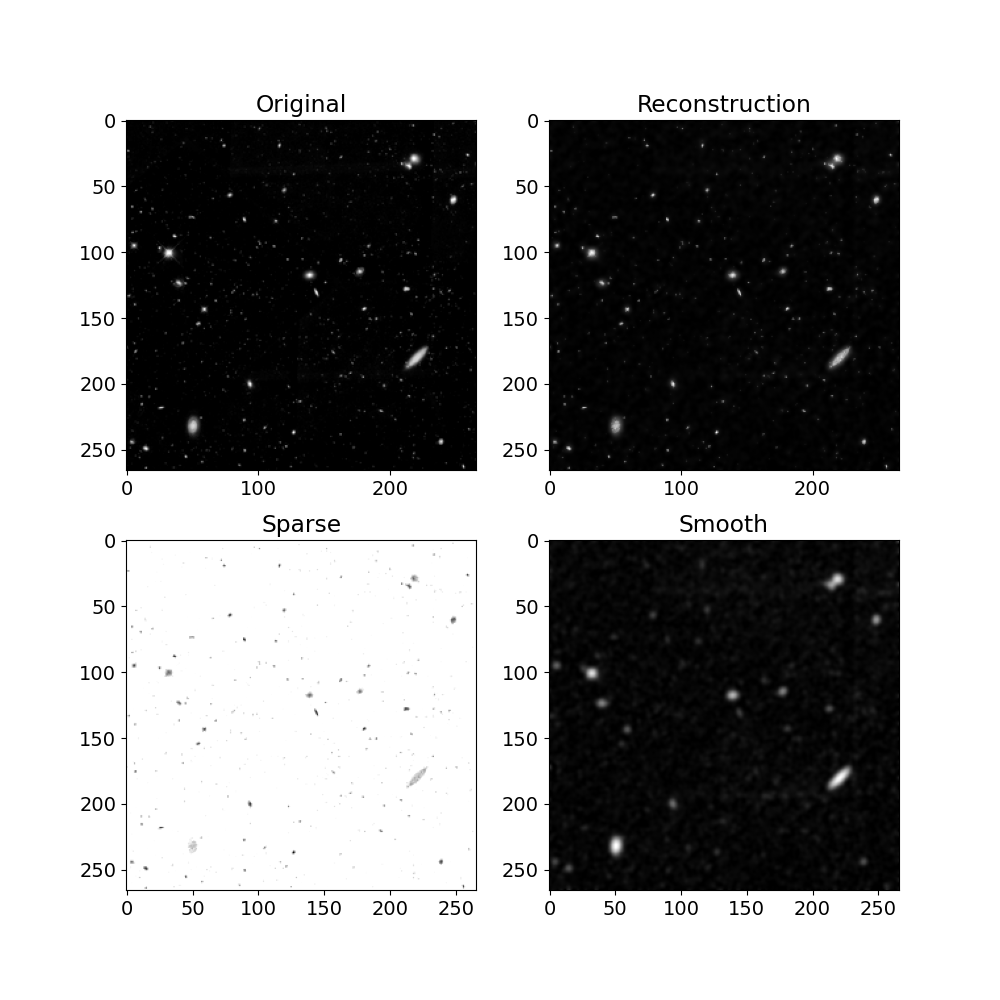
\includegraphics[width=1.7\textwidth]{h1.png}}
    \caption{Reconstruction of a real low dimensional image with $\lambda_1 = 0.01$ and $\lambda_2 = 0.2$}
    \label{fig:h1}
\end{figure}

\begin{figure}
    \centering
    \makebox[\linewidth]{
        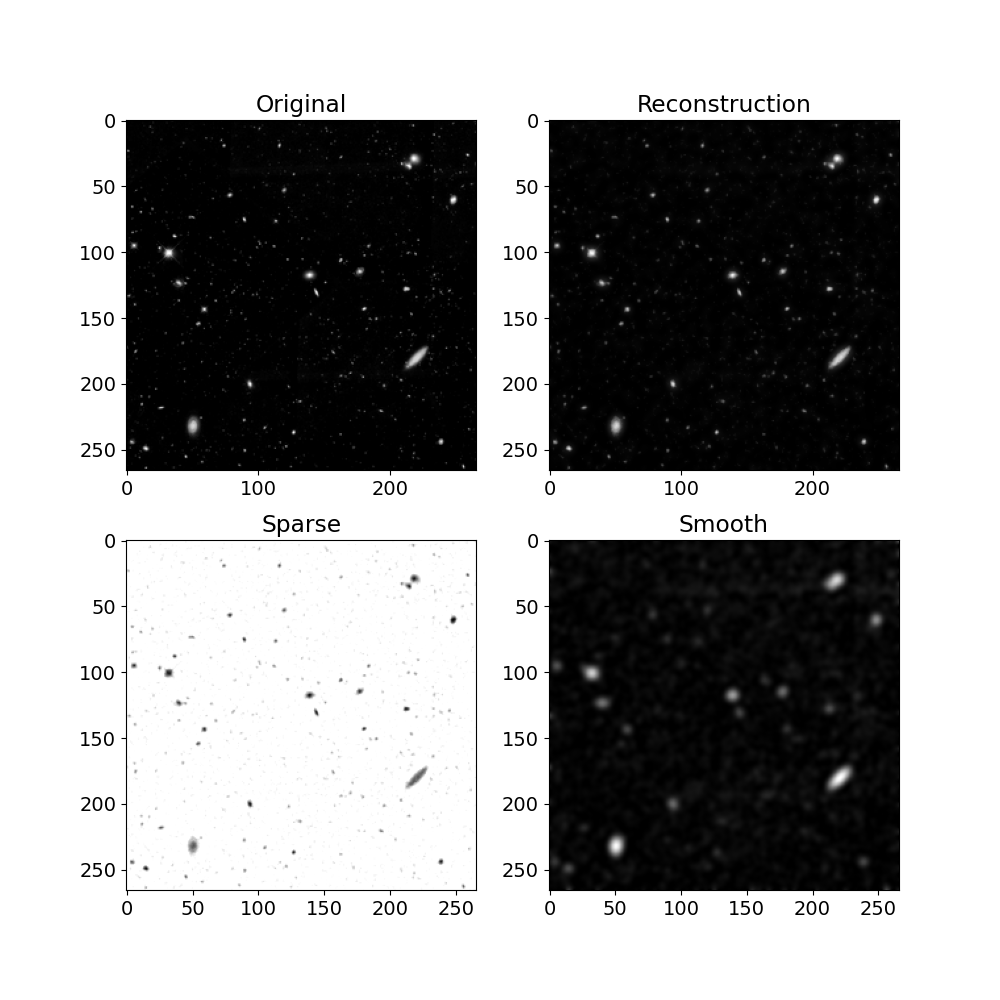
\includegraphics[width=1.7\textwidth]{h2.png}}
    \caption{Reconstruction of a real low dimensional image with $\lambda_1 = 0.001$ and $\lambda_2 = 0.2$}
    \label{fig:h2}
\end{figure}

In this section we apply our frame work on some real-world images. These images are taken from \href{https://hubblesite.org/resource-gallery/images}{hubblesite.org} which has a collection of images taken by the telescope hubble. All the reconstruct are done in the same settings with the subsampling of 10\% of the pixel with the method "Gaussian + Uniform" and without noise. The original image is gray scaled to the range 0-1. We have plotted four image each time, with the original image on top, at his right the reconstructed image $\boldsymbol{x} = \boldsymbol{x}_1 + \boldsymbol{x}_2$ and on bottom the two components, to better observe the sparse component we plot it with inverted colors.

We start with a low dimensional image to test the right tuning parameters on Figure \ref{fig:h7}, \ref{fig:h1}, \ref{fig:h2}. We see in all cases that the reconstruct is clean and we can not see much difference from the original. The tuning parameters only influence what each component $\boldsymbol{x}_1$ and $\boldsymbol{x}_2$ are, and has not much impact on the overall reconstruction $\boldsymbol{x} = \boldsymbol{x}_1 + \boldsymbol{x}_1$. 

For sparse and smooth component, we can not well separate the smooth extended light sources from the sparse and punctual ones, as we have with the simulated signal, we still see the punctual sources on the smooth component.  As for more spread ones, we can clearly see them on the smooth image and have a lower intensity on the sparse component. With a lower $\lambda_1$ we have another separation, on the sparse image we have the location of each sources and their shape, as for the smooth one we see spreadness of light for each source. 

To sum up, the sparse component captures the details while the smooth one gets the high level outline. For this reason, this reconstruct we need a low $\lambda_1$ compare to $\lambda_2$ since the sparse component has a lot more non-zero values than with the simulated signal. If we decrease $\lambda_1$ we have more details on the sparse component shown on Figure \ref{fig:h2}. While with a bigger $\lambda_1$ with have an image that is sparser.

Now we try the same reconstruct on the full higher dimensional image shown on Figure \ref{fig:h3}. We have the same result as with the low dimensional case. We see that the sparse component can extract the punctual sources and the smooth one that still has some residual. Then on Figure \ref{fig:h8}, \ref{fig:h6}, \ref{fig:h4} we have another high dimensional image, the same conclusion comes from these. 

We also tried with noisy measurements on Figure \ref{fig:h1n} and \ref{fig:h2n}. We see that we can reconstruct the biggest extended light sources in the smooth component, especially on Figure \ref{fig:h1n}. On Figure \ref{fig:h2n} we can see the three main  sources, with mostly noise on the rest. The sparse component is hard to analyse, but in the first Figure we can somehow see some punctual source that can be recover, those with the highest values. For example the punctual source on the bottom-right that appears clearly.

To conclude, the framework works well on real-world images. The only problem is to separate the punctual sources from the expended ones, we need the punctual sources to be represented as one or very few pixels. Apart from that, the smooth component easily reconstruct the rest of the image. With noise we notice the same proprieties as with the simulated signal, that we can recover the form of the smooth component and the highest values peaks on the sparse one.

\begin{figure}
    \centering
    \makebox[\linewidth]{
        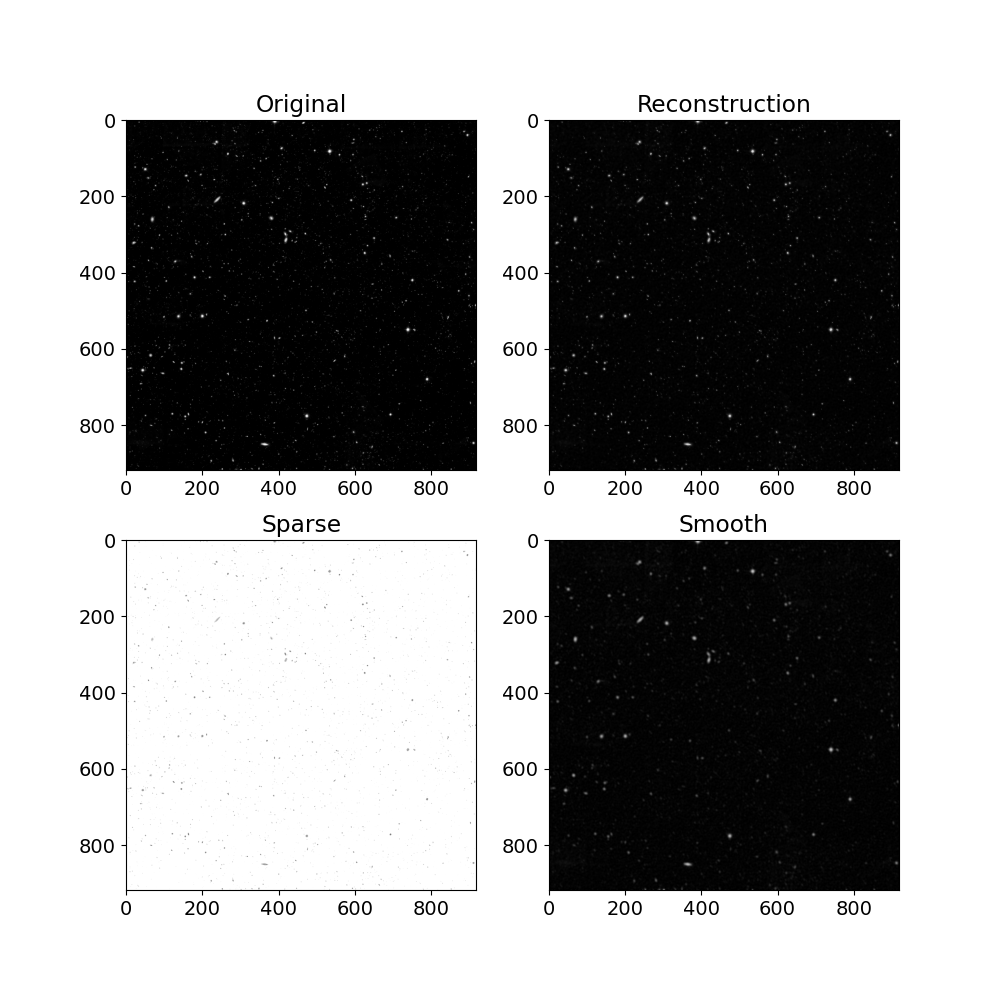
\includegraphics[width=1.7\textwidth]{h3.png}}
    \caption{Reconstruction of a real high dimensional image with $\lambda_1 = 0.01$ and $\lambda_2 = 0.2$}
    \label{fig:h3}
\end{figure}

\begin{figure}
    \centering
    \makebox[\linewidth]{
        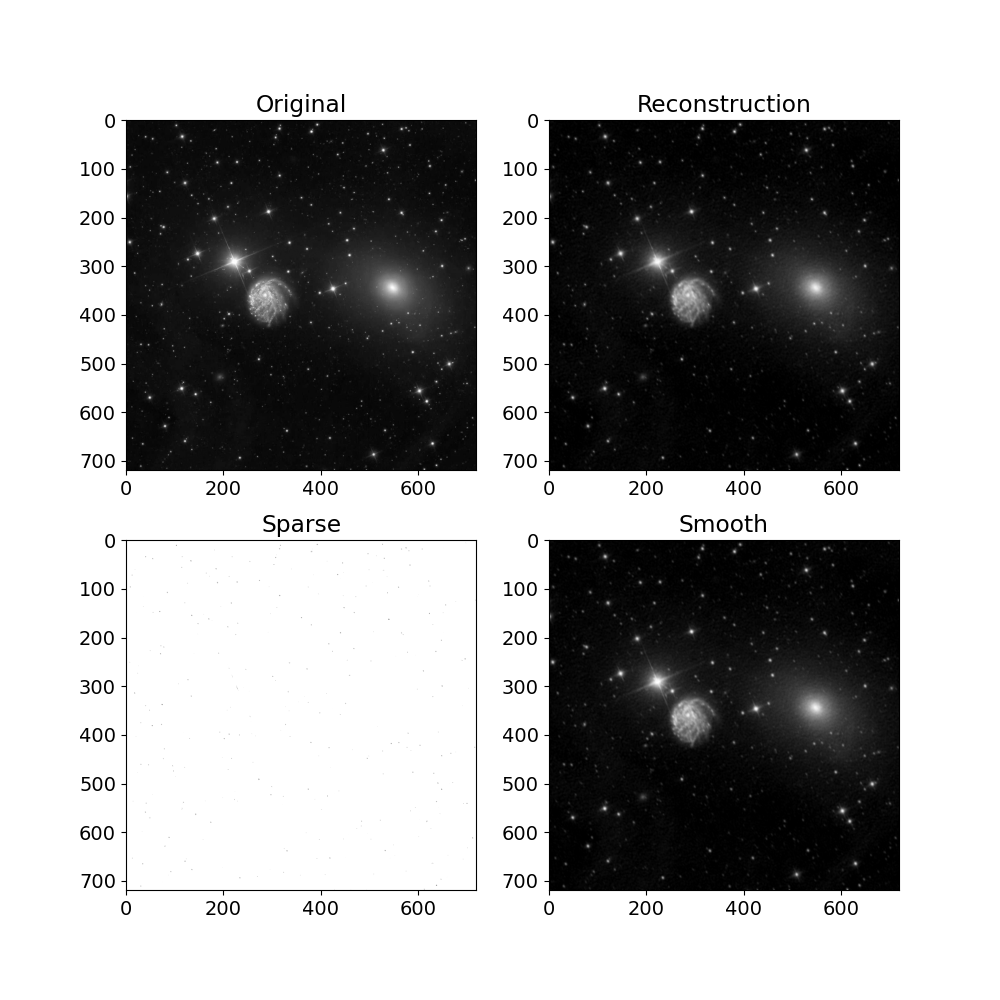
\includegraphics[width=1.7\textwidth]{h8.png}}
    \caption{Reconstruction of a real high dimensional image with $\lambda_1 = 0.02$ and $\lambda_2 = 0.06$}
    \label{fig:h8}
\end{figure}

\begin{figure}
    \centering
    \makebox[\linewidth]{
        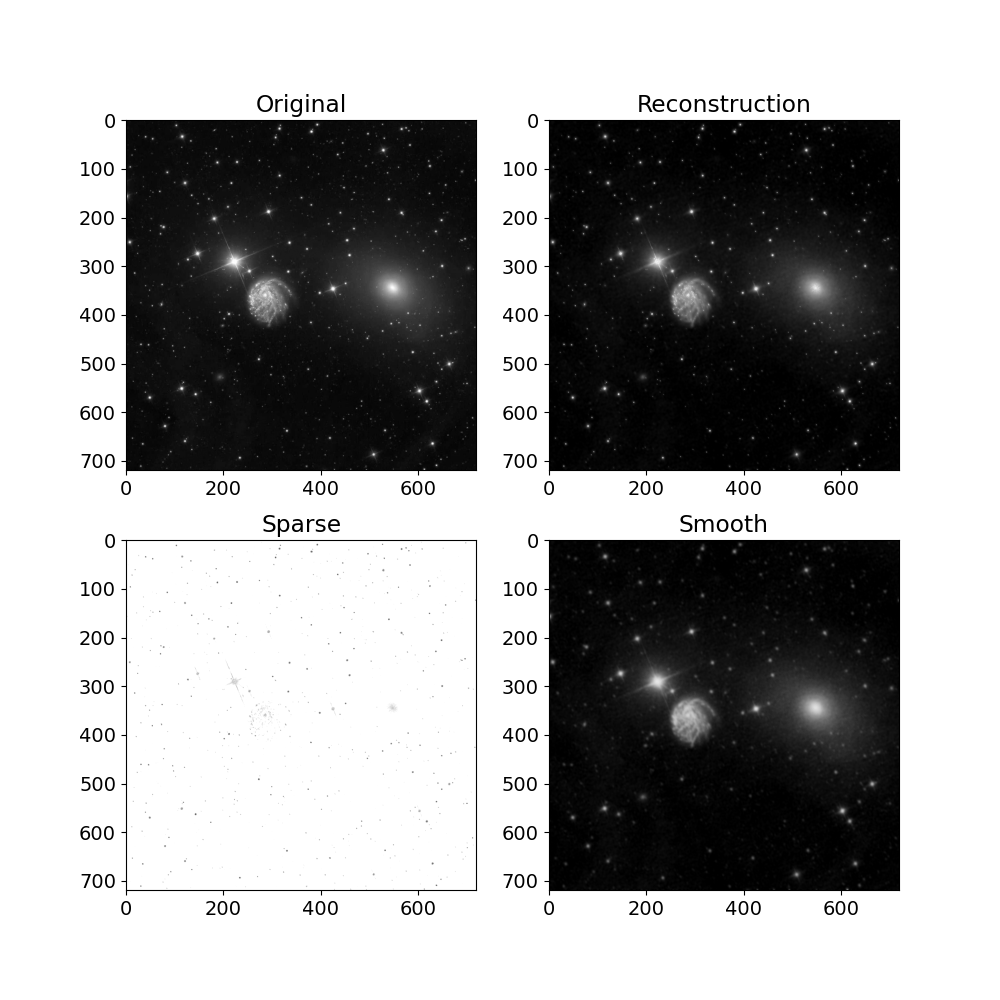
\includegraphics[width=1.7\textwidth]{h6.png}}
    \caption{Reconstruction of a real high dimensional image with $\lambda_1 = 0.01$ and $\lambda_2 = 0.2$}
    \label{fig:h6}
\end{figure}

\begin{figure}
    \centering
    \makebox[\linewidth]{
        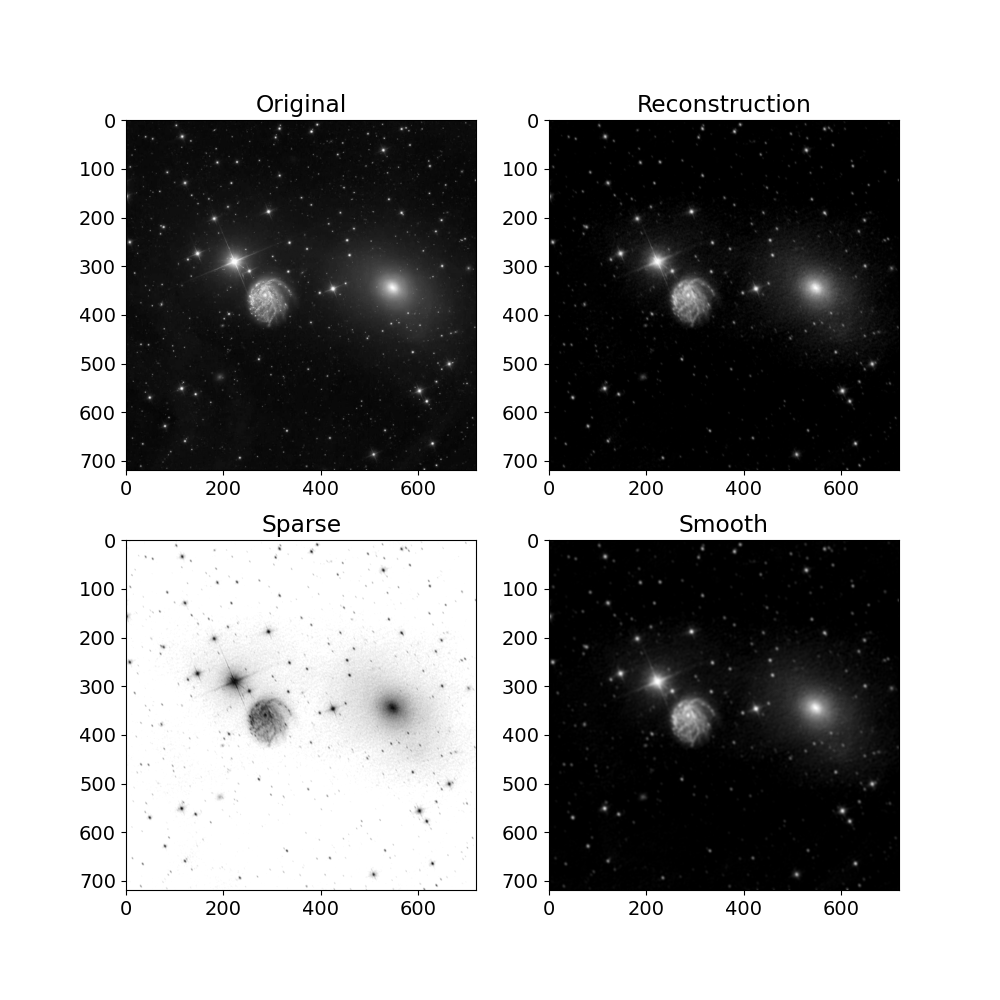
\includegraphics[width=1.7\textwidth]{h4.png}}
    \caption{Reconstruction of a real high dimensional image with $\lambda_1 = 0.001$ and $\lambda_2 = 0.2$}
    \label{fig:h4}
\end{figure}

\begin{figure}
    \centering
    \makebox[\linewidth]{
        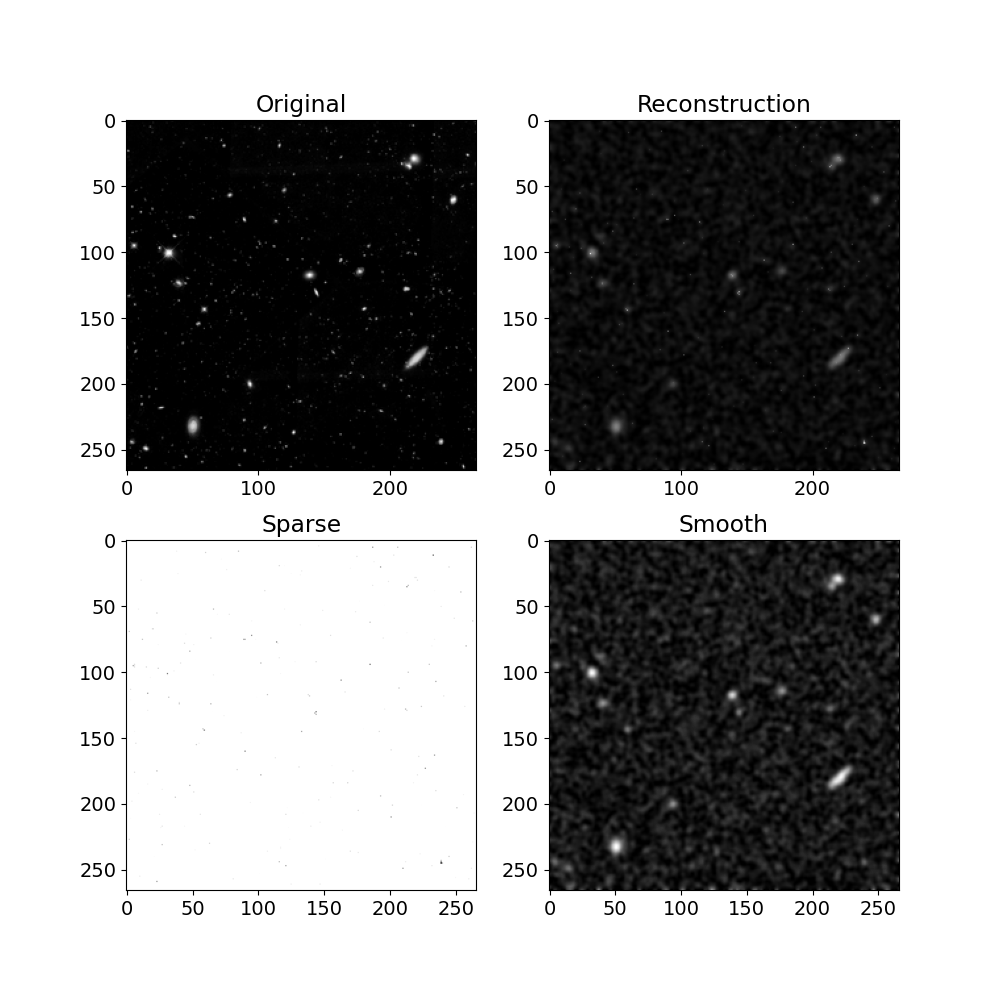
\includegraphics[width=1.7\textwidth]{h1n.png}}
    \caption{Reconstruction of a noisy real low dimensional image with PSNR = 10, $\lambda_1 = 0.2$ and $\lambda_2 = 1$}
    \label{fig:h1n}
\end{figure}

\begin{figure}
    \centering
    \makebox[\linewidth]{
        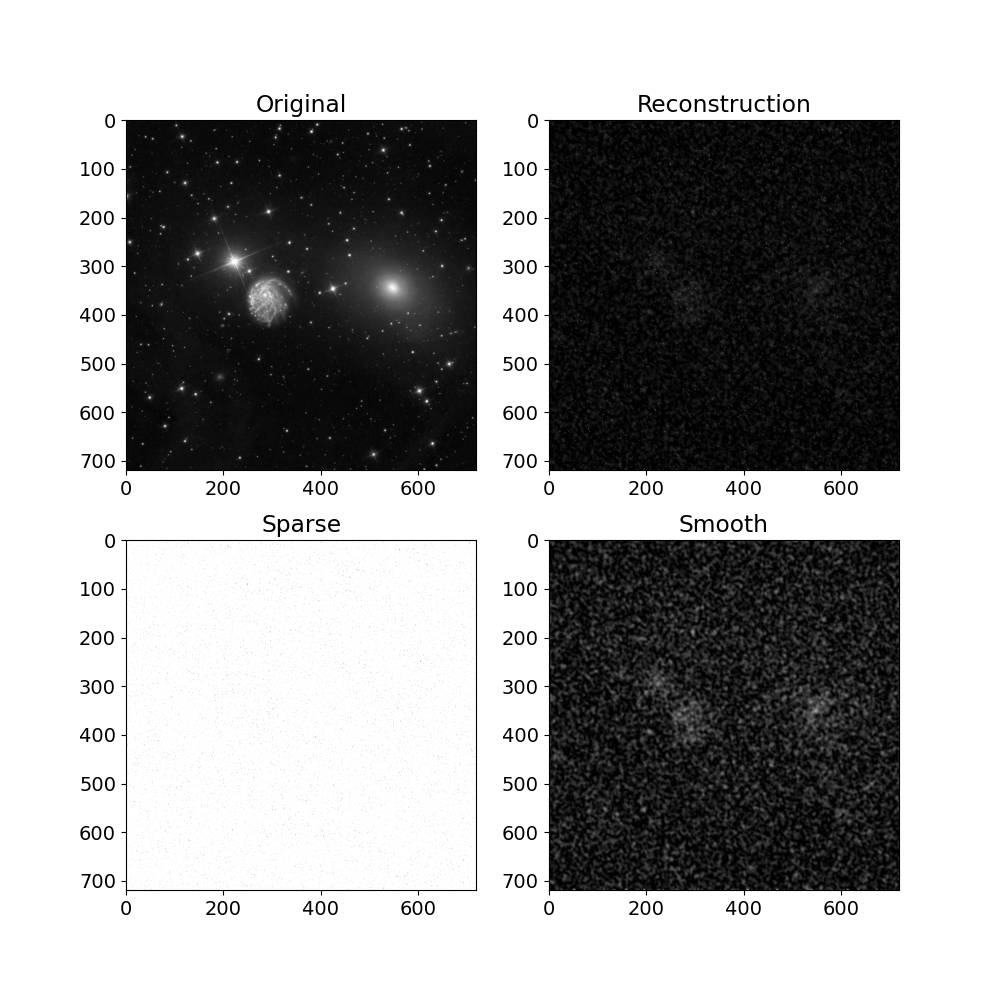
\includegraphics[width=1.7\textwidth]{h2n.png}}
    \caption{Reconstruction of a noisy real high dimensional image with PSNR = 20, $\lambda_1 = 0.2$ and $\lambda_2 = 1$}
    \label{fig:h2n}
\end{figure}


\chapter{Conclusion}
We have presented a framework for the reconstruction of sparse-plus-smooth images. The reconstruction is performed by solving a regularized minimization problem with a mixed penalty, using a subsampling of the 2D DFT. This is implemented with APGD with the help of the package pycsou in python. We have shown the efficacy of the framework on a simulated signal and see the influence of each parameter. We ended by testing the framework some real world image and saw that it can work well in some case and poorly in others.

The main Take-away message is that using a mixed penalty to reconstruct sparse-plus-smooth image is indeed a good idea and outperforms models that use a single penalty. On the practical side, implementing this regularized inverse problem with mixed penalty does not cost us more than classical models, with the help of the proximal algorithm, and is remarkably fast to compute. The only down side is that we got two tuning parameters that makes that model more complex and it is often really hard to find good $\lambda_1$, $\lambda_2$ values for a given level of noise, but also give more possibility on the from of each reconstructed component.

\addcontentsline{toc}{chapter}{Bibliography}
\bibliography{refs.bib}{}
\bibliographystyle{plain}

\end{document}
